\documentclass[fleqn,11pt,aspectratio=43]{beamer}
\usepackage[utf8x]{inputenc}
\usepackage[T1]{fontenc}
\usepackage[ngerman]{babel}
\usepackage{stmaryrd}
\usepackage{amsfonts}
\usepackage{amssymb}
\usepackage{amsmath}
\usepackage{microtype}

\usepackage{listings}
\usepackage{color}
\usepackage{pxfonts}

\definecolor{mygreen}{RGB}{51,141,120}
\definecolor{myblue}{RGB}{0,128,180}
\definecolor{myviolet}{RGB}{118,0,118}

\lstset{ %
  language=Haskell,
  backgroundcolor=\color{white},         % choose the background color
  basicstyle=\ttfamily\footnotesize,     % size of fonts used for the code
  numbers=none,
  breaklines=true,                       % automatic line breaking only at whitespace
  captionpos=b,                          % sets the caption-position to bottom
  commentstyle=\color{mygreen},    % comment style
  escapeinside={\%*}{*)},                % if you want to add LaTeX within your code
  keywordstyle=\color{myblue}\bfseries, % keyword style
  stringstyle=\color{myviolet},    % string literal style
  frame=single,
  tabsize=2
}
\usepackage{tikz}
\usetikzlibrary{
  arrows,
  shapes.misc,
  shapes.arrows,
  chains,
  matrix,
  positioning,
  scopes,
  decorations.pathmorphing,
  shadows,
  backgrounds
}


\usetheme[%
  %cmyk,%<cmyk/rgbprint>,          Auswahl des Farbmodells
  orange,%<blue/orange/green/violet> Auswahl des Sekundärfarbklangs
  %dark,%<light,medium>        Auswahl der Helligkeit
  %colorhead,%    Farbig hinterlegte Kopfleiste
  %colorfoot,%    Farbig hinterlegt Fußleiste auf Titelseite
  %colorblocks,%   Blöcke Farbig hinterlegen
  %nopagenum,%    Keine Seitennumer in Fußzeile
  %nodate,%       Kein Datum in Fußleiste
  %tocinheader,%   Inhaltsverzeichnis in Kopfleiste
  %tinytocinheader,% kleines Kopfleisten-Inhaltsverzeichnis
  %widetoc,%      breites Kopfleisten-Inhaltsverzeichnis
  %narrowtoc,%    schmales Kopfleisten-Inhaltsverzeichnis
  %nosubsectionsinheader,%  Keine subsections im Kopfleisten-Inhaltsverzeichnis
  %nologoinfoot,% Kein Logo im Fußbereich darstellen
  ]{tubs}

\titlegraphic[scaled]{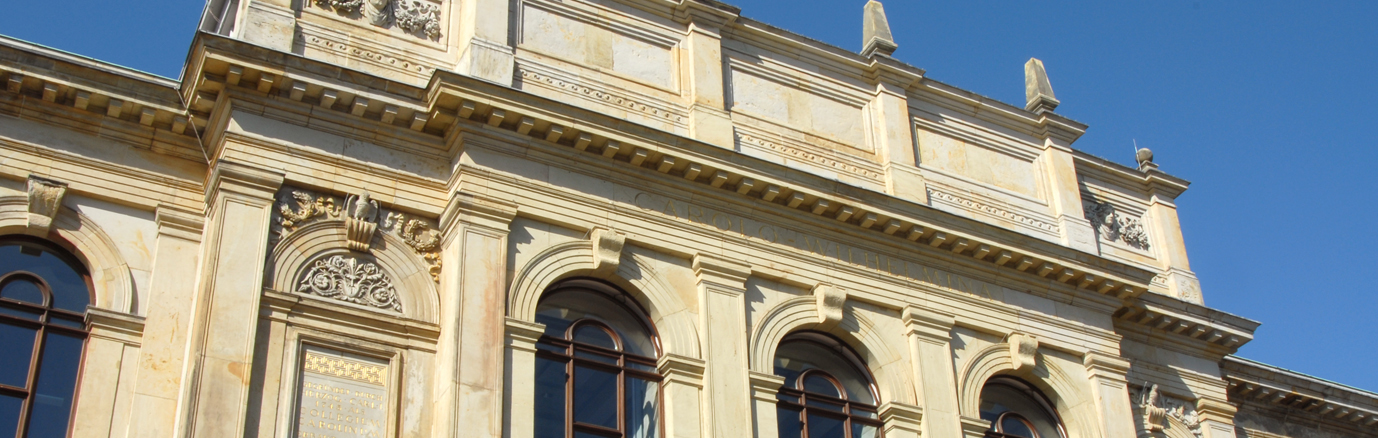
\includegraphics{img/titlepicture.jpg}}
\logo{
\includegraphics{img/logo_mit_text.pdf}}

\AtBeginSection[]{
  \begin{frame}[noframenumbering] 
  		\scriptsize
  		\frametitle{Überblick}  
  		\tableofcontents[currentsection, hideallsubsections]
  \end{frame}
}

\AtBeginSubsection[]{
  \begin{frame}[noframenumbering]
    	\scriptsize 
  		\frametitle{\insertsectionhead - \insertsubsectionhead} 
  		\tableofcontents[ 
  			currentsubsection, 
  		    sectionstyle=show/hide, 
  		   	subsectionstyle=show/shaded/hide] 
  \end{frame}
}


\title{Programmieren für Fortgeschrittene - \\eine Einführung in Haskell}

\author[Stephan Mielke]{\emph{Stephan Mielke}}
\institute[TU Braunschweig, IPS]{Technische Universität Braunschweig, IPS}


\begin{document}

\subtitle{Teil eins - Was ist Haskell} 
\date{17.11.2014}

\begin{frame}[plain, noframenumbering]
\titlepage
\end{frame}

\begin{frame}[noframenumbering]
  \scriptsize
  %\frametitle{\insertsectionhead}  
  \frametitle{Überblick}  
  %\begin{block}{\vspace*{-2ex}}
    \tableofcontents[currentsection,sectionstyle=show, hideallsubsections]
  %end{block} 
\end{frame}

\section*{Organisatorisches~}
\begin{frame}
\frametitle{Organisatorisches}
\begin{block}{\vspace*{-2ex}}
	\begin{itemize}
	  \item Jeweils Montags von 9:45 - 11:15 in IZ 261 (IPS Terminal Raum)
	  \item 5 / 6 Termine am:
	  \begin{itemize}
	  \item Fest: 17.11.2014, 01.12.2014, 15.12.2014
	  \item Variabel: 12.01.2015, 26.01.2015
	  \item Oder: 05.01.2015, 19.01.2015, 02.02.2015
	  \end{itemize}
	  \item Heute komplett \glqq Vorlesung\grqq, sonst 30-45 Minuten und danach Übung 
	\end{itemize}
\end{block}
\end{frame}

\begin{frame}
\frametitle{Quellen}
\begin{block}{\vspace*{-2ex}}	
	\begin{itemize}
	  \item Algorithmieren und Programmieren\\ Vorlesung von Prof. Dr. Petra Hofstedt (BTU)
	  \item Moderne Funktionale Programmierung \\ Vorlesung von Prof. Dr. Petra Hofstedt (BTU)
	  \item Eine Einführung in die funktionale Programmierung mit Haskell \\ Übungsskript zu unserer Vorlesung
	  \item Haskell - Intensivkurs
	\end{itemize}
\end{block}
\end{frame}

\section{Das funktionale Paradigma~}
\begin{frame}
\frametitle{Paradigmen}
\begin{block}{\vspace*{-2ex}}
\begin{itemize}
  \item Programmierparadigma\\
		Generelle Sicht bei der Modellierung und Lösung eines Problems
  \item Klassische Unterscheidung
  \begin{itemize}
    \item Imperative Sprachen\\
    	 \textbf{"`Wie"'} findet die Lösung statt\\
    	 Folge von \emph{Anweisungen} zur Problemlösung  
    \item Deklarative Sprachen \\
    	 \textbf{"`Was"'} ist die Lösung \\
    	 \emph{Deklarative Beschreibung} der Lösung bzw. des Problems
  \end{itemize}
\end{itemize}
\end{block}
\end{frame}

\begin{frame}
\frametitle{Paradigmen}
\begin{center}
\begin{tikzpicture}[>=stealth',shorten >=1pt,auto,node distance=2.5cm, xscale=2]
\node (Paradigmen)	{Paradigmen};
\node (imperativ) [below left of = Paradigmen]	{imperativ};
\node (prozedural) [below left of = imperativ]	{prozedural};
\node (oo) [below of = Paradigmen]	{objekt-orientiert};
\node (deklarativ) [below right of = Paradigmen]	{deklarativ};
\node (fl) [below left of = deklarativ]	{funktional-logisch};
\node (cl) [below right of = deklarativ]	{constraint-logisch};
\node (funktional) [below left of = fl]	{\textbf{funktional}};
\node (logisch) [right of = funktional]	{logisch};
\node (cb) [right of = logisch]	{constraint-basiert};

\path	(Paradigmen)	edge node { } (imperativ)
							edge node { } (deklarativ)
			(imperativ)		edge node { } (prozedural)
			(deklarativ)	edge node { } (fl)
							edge node { } (cl)
			(fl)			edge node { } (funktional)
							edge node { } (logisch)
			(cl)			edge node { } (logisch)
							edge node { } (cb);

\path[dashed]	(Paradigmen)	edge node { } (oo)
			(imperativ)		edge node { } (oo);		
\end{tikzpicture}
\end{center}
\end{frame}

\begin{frame}
\frametitle{Funktionale Paradigma}
\begin{block}{\vspace*{-2ex}}
\begin{itemize}
  \item Hohes Abstraktionsniveau \\ 
  Klare Darstellung der Programmiertechniken und Algorithmen,
d.h. Konzentration auf die Konzepte statt auf die Sprache
  \item Klare, elegante und kompakte Programme \\ 
  Kurze Entwicklungszeiten, lesbare Programme
  \item Keine Seiteneffekte \\ 
  Erleichtert Verstehen, Optimierung, Verifikation
  \item Saubere theoretische Fundierung \\ 
  Ermöglicht Verifikation und erleichtert formale Argumentation über Programme
\end{itemize}
\end{block}
\end{frame}

\section{Haskell~}
\begin{frame}
\frametitle{Haskell}
\begin{block}{\vspace*{-2ex}}
\begin{itemize}
  \item 1990 als Haskell 1.0 veröffentlicht
  \item Aktuelle Version Haskell 2010
  \item An Haskell 2014 (Preview) wird (immer noch) \glqq gearbeitet\grqq
\end{itemize}
\end{block}
\end{frame}

\begin{frame}[fragile]
\frametitle{Hello World} 
\begin{lstlisting}
module Main where
 
main :: IO ()
main = putStrLn "Hello, World!"
\end{lstlisting}
\pause
\begin{block}{Ausgabe}
\begin{center}
Hello, World!
\end{center}
\end{block}
\end{frame}

\begin{frame}
\frametitle{Haskell Compiler}
\begin{block}{\vspace*{-2ex}}
\begin{itemize}
  \item Hugs (Haskell User's Gofer System) \\ Implementiert Haskell 98 \\ Seit ca 6 Jahren nicht weiterentwickelt
  \item Yhc (York Haskell Compiler) \\ Implementiert Haskell 98 \\ Projekt eingestellt
  \item GHC (Glasgow Haskell Compiler) \\ Implementiert Haskell 98 / 2010 \\ Weit verbreitster Haskell Compiler \\ 
  Besitzt den GHCi als Haskell Interpreter
\end{itemize}
\end{block}
\end{frame}

\begin{frame}
\frametitle{Glasgow Haskell Compiler}
\begin{block}{\vspace*{-2ex}}
\begin{itemize}
  \item Original Prototyp '89 in LML (Lazy ML) 
  \item Bei der Entwicklung von Haskell in Haskell (API) neu geschrieben ('89)
  \item Nur kleine Teile in C bzw. C-\,-\  (C verwandte Sprache zur Nutzung als Zwischencode)
  \item Erweitert den Haskell Standard um noch nicht standardisierte Erweiterungen
  \item Plattform und Architektur \glqq fast\grqq\ unabhängig
  \item Vergleichbar mit Java
  \begin{itemize}
  	\item JVM in C bzw. C++
  	\item API in Java
  	\item Bytecode als Zwischencode
  \end{itemize}
\end{itemize}
\end{block}
\end{frame}

\begin{frame}
\frametitle{Laufzeitumgebung}
\begin{block}{\vspace*{-2ex}}
\begin{itemize}
  \item Wenn das Programm in Maschinencode übersetzt wurde, wird keine externe Laufzeitumgebung benötigt (nativer Code)\\
  		die "`Laufzeitumgebung"' wird mit in das Programm gepackt
  \item Bei Benutzung des Interpreters wird dieser als Laufzeitumgebung verwendet.
\end{itemize}
\end{block}
\end{frame}

\begin{frame}
\frametitle{Interne Funktionsweise}
\begin{block}{\vspace*{-2ex}}
\begin{itemize}
  \item Erzeugung von Zwischencode "`C-\,-"'
  \item C-\,-\  ist wie C-Code jedoch "`etwas"' anders
  \item Dieser Code wird optimiert und weiter compiliert
  \item "`-fasm"' erzeugt Maschinencode (Standard)
  \item "`-fvia-C"' erzeugt C-Code aus C-\,-\ \\
  		Seit Version 7.0 nicht mehr unterstützt
  \item "`-fllvm"' nutzt den LLVM als Backend-Compiler
\end{itemize}
\end{block}
\end{frame}

\begin{frame}
\frametitle{Interne Funktionsweise}
\begin{figure}
\centering
\includegraphics*[scale=0.4]{images/HscPipe2_1}
\caption{Compiler Teil 1 \copyright \url{haskell.org}}
\end{figure}
\end{frame}


\begin{frame}[noframenumbering]
\frametitle{Interne Funktionsweise}
\begin{figure}
\centering
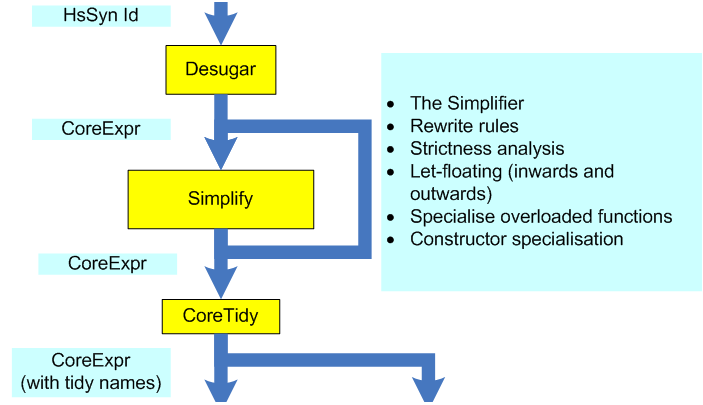
\includegraphics[scale=0.4]{images/HscPipe2_2.png}
\caption{Compiler Teil 2 \copyright \url{haskell.org}}
\end{figure}
\end{frame}

\begin{frame}[noframenumbering]
\frametitle{Interne Funktionsweise}
\begin{figure}
\centering
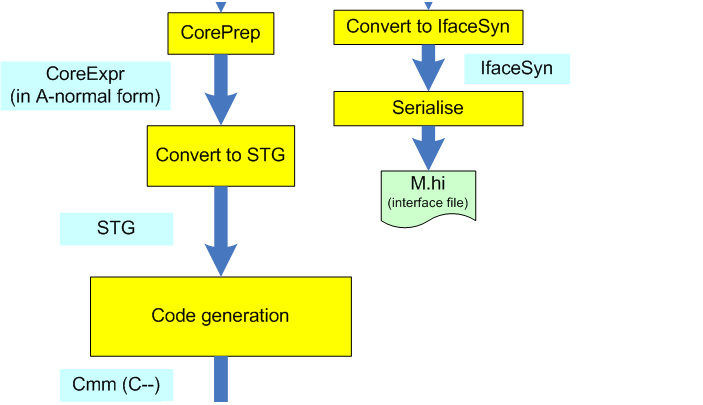
\includegraphics[scale=0.4]{images/HscPipe2_3.png}
\caption{Compiler Teil 3 \copyright \url{haskell.org}}
\end{figure}
\end{frame}

\begin{frame}[noframenumbering]
\frametitle{Interne Funktionsweise}
\begin{figure}
\centering
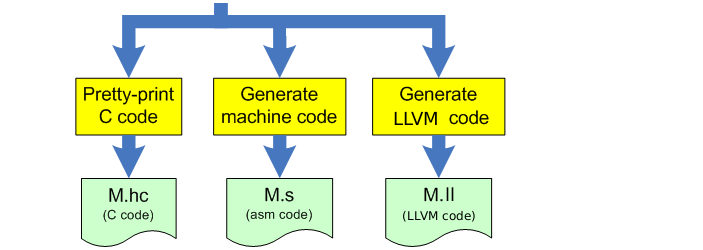
\includegraphics[scale=0.4]{images/HscPipe2_4.png}
\caption{Compiler Teil 4 \copyright \url{haskell.org}}
\end{figure}
\end{frame}

\section{Semantische Grundbegriffe~}

\subsection{Namen und Attribute}
\begin{frame}
\frametitle{Namen und Attribute}
\begin{block}{\vspace*{-2ex}}
\begin{itemize}
  \item Alle endlichen ASCII-Strings außer:
  \\ \lstinline|case|, \lstinline|class|, \lstinline|data|, \lstinline|default|, \lstinline|deriving|, \lstinline|do|, \lstinline|else|, \lstinline|if|, \lstinline|import|, \lstinline|in|, \lstinline|infix|, \lstinline|infixl|, \lstinline|infixr|, \lstinline|instance|, \lstinline|let|, \lstinline|module|, \lstinline|newtype|, \lstinline|of|, \lstinline|then|, \lstinline|type|, \lstinline|where|
  \item Bezeichner sind case-sensitiv (\lstinline|pLus| $\neq$ \lstinline|plus|) 
  \item \lstinline|_| (Unterstrich) ist der Platzhalter
  \item Module beginnen mit einem Großbuchstaben
  \item Funktionen mit einem Kleinbuchstaben
\end{itemize}
\end{block}
\end{frame}

\subsection{Variablen und Konstanten}
\begin{frame}
\frametitle{Variablen}
\begin{block}{\vspace*{-2ex}}
\begin{itemize}
  \item Globale Variablen existieren nicht
  \item Lokale Variablen existieren nur in Funktionen als Teilergebnis
\end{itemize}
\end{block}
\end{frame}

\begin{frame}
\frametitle{Konstanten}
\begin{block}{\vspace*{-2ex}}
\begin{itemize}
  \item Konstanten sind Funktionen ohne Parameter
  \item Mathematisch: $\emptyset \to |W_f| = 1$
\end{itemize}
%Konstanten sind Funktionen ohne Parameter
\end{block}
\end{frame}

\subsection{Ausdrücke}
\begin{frame}
\frametitle{Ausdrücke}
\begin{block}{\vspace*{-2ex}}
Elementare Ausdrücke bzw. Grundterme setzen sich zusammen aus:
\begin{itemize}
  \item Konstanten wie z.B. Zahlen (\lstinline|10|, \lstinline|9.8|), Zeichen (\lstinline|'a'|, \lstinline|'Z'|), \ldots
  \item Andere Funktionen \lstinline|sin|, \lstinline|+|, \lstinline|*|, \ldots
\end{itemize}
\end{block}
\begin{alertblock}{Infixnotation}
Funktionszeichen: \lstinline|3 + 4| $\equiv$ \lstinline|(+) 3 4|\\
Funktionsname: \lstinline|mod 100 4| $\equiv$ \lstinline|100 `mod` 4|
\end{alertblock}
\end{frame}

\begin{frame}
\frametitle{Ausdrücke}
\begin{block}{\vspace*{-2ex}}
\begin{itemize}
  \item Elementare Ausdrücke mit Variablen sind Ausdrücke bzw. Terme
  \item Durch einen "`Vorspann"' wie $\ x$ wird die Variable $x$ mit der $\lambda$-Notation "`gebunden"'
  \item $\lambda a \to \lambda b \to a + b$ ist ein $\lambda$-Ausdruck
  \item $\lambda$ ist kein ASCII Zeichen, deswegen wird "`\textbackslash"' verwendet 
\end{itemize}
\end{block}
\end{frame}

\begin{frame}[fragile]
\frametitle{Ausdrücke} 
\begin{exampleblock}{Elementarer Ausdruck}
\begin{lstlisting}
plus = 10 + 30
\end{lstlisting}
\end{exampleblock}
\begin{exampleblock}{Ausdruck}
\begin{lstlisting}
plus' a b = a + b
\end{lstlisting}
\end{exampleblock}
\begin{exampleblock}{Lambda ($\lambda$)-Ausdruck}
\begin{lstlisting}
plus'' =  \a -> \b -> a + b
\end{lstlisting}
\end{exampleblock}
\end{frame}

\subsection{Funktionen}
\begin{frame}
\frametitle{Deklaration von Funktionen}
\begin{block}{\vspace*{-2ex}}
\begin{itemize}
  \item Funktion $f$ ist ein Tripel $(D_f, W_f, R_f)$
  \item $D_f$ Definitionsmenge
  \item $W_f$ Wertemenge
  \item $R_f \subseteq D_f \times W_f$
  \item $R_f$ muss \textbf{rechtseindeutig} sein, d.h. es gibt keine zwei Paare $(a,b_1) \in R_f$ und $(a,b_2) \in R_f$ mit $b_1 \neq b_2$
  \item Somit gilt: eine Funktion $f$ bildet den Argumentwert $x$ in den Resultatwert $y$ ab 
\end{itemize}
\end{block}
\end{frame}

\begin{frame}
\frametitle{Deklaration von Funktionen}
\only<1>{
\vspace*{-1ex}
\begin{exampleblock}{Konstante}
\begin{center}
\scalebox{0.6}{\begin{tikzpicture}[
      nonterminal/.style={
         rectangle,
         minimum size=5.0mm,
         very thick,
         draw=blue!50!black!50,
         top color=white,
         bottom color=blue!50!black!20,
         font=\itshape\scriptsize,
         %text height=1.5ex,
         %text depth=.25ex
      },
      terminal/.style={
         rounded rectangle,
         minimum size=5.0mm,
         very thick,draw=black!50,
         top color=white,bottom color=black!20,
         font=\ttfamily\scriptsize,
         %text height=1.5ex,
         %text depth=.25ex
      },
      skip loop/.style={
         to path={-- ++(0,#1) -| (\tikztotarget)}
      },
      point/.style={coordinate},>=stealth',thick,draw=black!50,
      tip/.style={->,shorten >=0.007pt},every join/.style={rounded corners},
      hv path/.style={to path={-| (\tikztotarget)}},
      vh path/.style={to path={|- (\tikztotarget)}},
      %text height=1.5ex,text depth=.25ex
    ]
    \matrix[column sep=5.0mm, row sep=3.0mm] {
 &  & \node (n13) [nonterminal] {Bezeichner}; & \node (n14) [terminal] {::}; & \node (n15) [nonterminal] {Typ Erg}; & \node (n16) [terminal] {LF}; &  & \\
\node (n21) [circle, draw, inner sep=0pt, minimum size=0.75ex] {}; & \node (n22) [point] {}; &  &  &  &  & \node (n27) [point] {}; & \node (n28) [point] {};\\
 &  & \node (n33) [point] {}; &  &  &  &  & \\
 &  &  &  &  &  &  & \\
 &  &  &  & \node (n55) [nonterminal] {Wert}; &  &  & \\
\node (n61) [point] {}; & \node (n62) [nonterminal] {Bezeichner}; & \node (n63) [terminal] {=}; & \node (n64) [point] {}; &  & \node (n66) [point] {}; & \node (n67) [terminal] {LF}; & \node (n68) [circle, draw, inner sep=0pt, minimum size=0.75ex] {};\\
 &  &  &  & \node (n75) [nonterminal] {Ausdruck}; &  &  & \\
    };
  { [start chain]
       \chainin (n21);
       \chainin (n22)    [join];
  }
  { [start chain]
       \chainin (n22);
       \chainin (n13)    [join=by {vh path,tip}];
  }
  { [start chain]
       \chainin (n13);
       \chainin (n14)    [join=by tip];
  }
  { [start chain]
       \chainin (n14);
       \chainin (n15)    [join=by tip];
  }
  { [start chain]
       \chainin (n15);
       \chainin (n16)    [join=by tip];
  }
  { [start chain]
       \chainin (n16);
       \chainin (n27)    [join=by {hv path}];
  }
  { [start chain]
       \chainin (n22);
       \chainin (n33)    [join=by {vh path}];
  }
  { [start chain]
       \chainin (n33);
       \chainin (n27)    [join=by {hv path}];
  }
  { [start chain]
       \chainin (n27);
       \chainin (n28)    [join=by tip];
  }
  { [start chain]
       \chainin (n61);
       \chainin (n62)    [join=by tip];
  }
  { [start chain]
       \chainin (n62);
       \chainin (n63)    [join=by tip];
  }
  { [start chain]
       \chainin (n63);
       \chainin (n64)    [join];
  }
  { [start chain]
       \chainin (n64);
       \chainin (n55)    [join=by {vh path,tip}];
  }
  { [start chain]
       \chainin (n55);
       \chainin (n66)    [join=by {hv path}];
  }
  { [start chain]
       \chainin (n64);
       \chainin (n75)    [join=by {vh path,tip}];
  }
  { [start chain]
       \chainin (n75);
       \chainin (n66)    [join=by {hv path}];
  }
  { [start chain]
       \chainin (n66);
       \chainin (n67)    [join=by tip];
  }
  { [start chain]
       \chainin (n67);
       \chainin (n68)    [join=by tip];
  }
\end{tikzpicture}
}
\end{center}
\end{exampleblock}}
\only<2>{
\vspace*{-1ex}
\begin{exampleblock}{Funktion}
\begin{center}
\scalebox{0.5}{\begin{tikzpicture}[
      nonterminal/.style={
         rectangle,
         minimum size=5.0mm,
         very thick,
         draw=blue!50!black!50,
         top color=white,
         bottom color=blue!50!black!20,
         font=\itshape\scriptsize,
         %text height=1.5ex,
         %text depth=.25ex
      },
      terminal/.style={
         rounded rectangle,
         minimum size=5.0mm,
         very thick,draw=black!50,
         top color=white,bottom color=black!20,
         font=\ttfamily\scriptsize,
         %text height=1.5ex,
         %text depth=.25ex
      },
      skip loop/.style={
         to path={-- ++(0,#1) -| (\tikztotarget)}
      },
      point/.style={coordinate},>=stealth',thick,draw=black!50,
      tip/.style={->,shorten >=0.007pt},every join/.style={rounded corners},
      hv path/.style={to path={-| (\tikztotarget)}},
      vh path/.style={to path={|- (\tikztotarget)}},
      %text height=1.5ex,text depth=.25ex
    ]
    \matrix[column sep=5.0mm, row sep=3.0mm] {
 &  &  &  &  & \node (n16) [point] {}; &  &  &  &  &  &  & \\
 &  & \node (n23) [nonterminal] {Bezeichner}; & \node (n24) [terminal] {::}; & \node (n25) [point] {}; & \node (n26) [nonterminal] {Typ Para}; & \node (n27) [terminal] {->}; & \node (n28) [point] {}; & \node (n29) [nonterminal] {Typ Erg}; & \node (n210) [terminal] {LF}; &  &  & \\
\node (n31) [circle, draw, inner sep=0pt, minimum size=0.75ex] {}; & \node (n32) [point] {}; &  &  &  &  &  &  &  &  & \node (n311) [point] {}; & \node (n312) [point] {}; & \\
 &  & \node (n43) [point] {}; &  &  &  &  &  &  &  &  &  & \\
 &  &  &  &  &  &  &  &  &  &  &  & \\
 &  &  &  &  &  & \node (n67) [point] {}; &  &  &  &  &  & \\
 &  &  &  & \node (n75) [point] {}; &  &  &  & \node (n79) [nonterminal] {Wert}; &  &  &  & \\
\node (n81) [point] {}; & \node (n82) [point] {}; & \node (n83) [nonterminal] {Bezeichner}; & \node (n84) [point] {}; & \node (n85) [nonterminal] {Bezeichner Para}; & \node (n86) [point] {}; & \node (n87) [terminal] {=}; & \node (n88) [point] {}; &  & \node (n810) [point] {}; & \node (n811) [terminal] {LF}; & \node (n812) [point] {}; & \node (n813) [circle, draw, inner sep=0pt, minimum size=0.75ex] {};\\
 &  &  &  &  &  &  &  & \node (n99) [nonterminal] {Ausdruck}; &  &  &  & \\
    };
  { [start chain]
       \chainin (n31);
       \chainin (n32)    [join];
  }
  { [start chain]
       \chainin (n32);
       \chainin (n23)    [join=by {vh path,tip}];
  }
  { [start chain]
       \chainin (n23);
       \chainin (n24)    [join=by tip];
  }
  { [start chain]
       \chainin (n24);
       \chainin (n25)    [join];
  }
  { [start chain]
       \chainin (n25);
       \chainin (n26)    [join=by tip];
  }
  { [start chain]
       \chainin (n26);
       \chainin (n27)    [join=by tip];
  }
  { [start chain]
       \chainin (n27);
       \chainin (n28)    [join];
  }
  { [start chain]
       \chainin (n28);
       \chainin (n29)    [join=by tip];
  }
  { [start chain]
       \chainin (n29);
       \chainin (n210)    [join=by tip];
  }
  { [start chain]
       \chainin (n210);
       \chainin (n311)    [join=by {hv path}];
  }
  { [start chain]
       \chainin (n32);
       \chainin (n43)    [join=by {vh path}];
  }
  { [start chain]
       \chainin (n43);
       \chainin (n311)    [join=by {hv path}];
  }
  { [start chain]
       \chainin (n311);
       \chainin (n312)    [join=by tip];
  }
  { [start chain]
       \chainin (n81);
       \chainin (n82)    [join];
  }
  { [start chain]
       \chainin (n82);
       \chainin (n83)    [join=by tip];
  }
  { [start chain]
       \chainin (n83);
       \chainin (n84)    [join];
  }
  { [start chain]
       \chainin (n84);
       \chainin (n85)    [join=by tip];
  }
  { [start chain]
       \chainin (n85);
       \chainin (n86)    [join];
  }
  { [start chain]
       \chainin (n86);
       \chainin (n87)    [join=by tip];
  }
  { [start chain]
       \chainin (n87);
       \chainin (n88)    [join];
  }
  { [start chain]
       \chainin (n88);
       \chainin (n79)    [join=by {vh path,tip}];
  }
  { [start chain]
       \chainin (n79);
       \chainin (n810)    [join=by {hv path}];
  }
  { [start chain]
       \chainin (n88);
       \chainin (n99)    [join=by {vh path,tip}];
  }
  { [start chain]
       \chainin (n99);
       \chainin (n810)    [join=by {hv path}];
  }
  { [start chain]
       \chainin (n810);
       \chainin (n811)    [join=by tip];
  }
  { [start chain]
       \chainin (n811);
       \chainin (n812)    [join];
  }
  { [start chain]
       \chainin (n812);
       \chainin (n813)    [join=by tip];
  }
  { [start chain]
       \chainin (n28);
       \chainin (n16)    [join=by vh path];
       \chainin (n25)    [join=by {hv path,tip}];
  }
  { [start chain]
       \chainin (n86);
       \chainin (n75)    [join=by vh path];
       \chainin (n84)    [join=by {hv path,tip}];
  }
  { [start chain]
       \chainin (n812);
       \chainin (n67)    [join=by vh path];
       \chainin (n82)    [join=by {hv path,tip}];
  }
\end{tikzpicture}
}
\end{center}
\end{exampleblock}}
\only<3>{\begin{exampleblock}{Allgemein}
\begin{center}
\scalebox{0.6}{\begin{tikzpicture}[
      nonterminal/.style={
         rectangle,
         minimum size=5.0mm,
         very thick,
         draw=blue!50!black!50,
         top color=white,
         bottom color=blue!50!black!20,
         font=\itshape\scriptsize,
         %text height=1.5ex,
         %text depth=.25ex
      },
      terminal/.style={
         rounded rectangle,
         minimum size=5.0mm,
         very thick,draw=black!50,
         top color=white,bottom color=black!20,
         font=\ttfamily\scriptsize,
         %text height=1.5ex,
         %text depth=.25ex
      },
      skip loop/.style={
         to path={-- ++(0,#1) -| (\tikztotarget)}
      },
      point/.style={coordinate},>=stealth',thick,draw=black!50,
      tip/.style={->,shorten >=0.007pt},every join/.style={rounded corners},
      hv path/.style={to path={-| (\tikztotarget)}},
      vh path/.style={to path={|- (\tikztotarget)}},
      %text height=1.5ex,text depth=.25ex
    ]
    \matrix[column sep=5.0mm, row sep=3.0mm] {
 &  &  &  &  & \node (n16) [terminal] {->}; & \node (n17) [nonterminal] {Typ Para}; &  &  &  &  &  & \\
 &  & \node (n23) [nonterminal] {Bezeichner}; & \node (n24) [terminal] {::}; & \node (n25) [point] {}; &  &  & \node (n28) [point] {}; & \node (n29) [nonterminal] {Typ Erg}; & \node (n210) [terminal] {LF}; &  &  & \\
\node (n31) [circle, draw, inner sep=0pt, minimum size=0.75ex] {}; & \node (n32) [point] {}; &  &  &  &  &  &  &  &  & \node (n311) [point] {}; & \node (n312) [point] {}; & \\
 &  & \node (n43) [point] {}; &  &  &  &  &  &  &  &  &  & \\
 &  &  &  &  &  &  &  &  &  &  &  & \\
 &  &  &  &  &  & \node (n67) [point] {}; &  &  &  &  &  & \\
 &  &  &  & \node (n75) [nonterminal] {Bezeichner Para}; &  &  &  & \node (n79) [nonterminal] {Wert}; &  &  &  & \\
\node (n81) [point] {}; & \node (n82) [point] {}; & \node (n83) [nonterminal] {Bezeichner}; & \node (n84) [point] {}; &  & \node (n86) [point] {}; & \node (n87) [terminal] {=}; & \node (n88) [point] {}; &  & \node (n810) [point] {}; & \node (n811) [terminal] {LF}; & \node (n812) [point] {}; & \node (n813) [circle, draw, inner sep=0pt, minimum size=0.75ex] {};\\
 &  &  &  &  &  &  &  & \node (n99) [nonterminal] {Ausdruck}; &  &  &  & \\
    };
  { [start chain]
       \chainin (n31);
       \chainin (n32)    [join];
  }
  { [start chain]
       \chainin (n32);
       \chainin (n23)    [join=by {vh path,tip}];
  }
  { [start chain]
       \chainin (n23);
       \chainin (n24)    [join=by tip];
  }
  { [start chain]
       \chainin (n24);
       \chainin (n25)    [join];
  }
  { [start chain]
       \chainin (n25);
       \chainin (n28)    [join];
  }
  { [start chain]
       \chainin (n17);
       \chainin (n16)    [join=by tip];
  }
  { [start chain]
       \chainin (n28);
       \chainin (n17)    [join=by {vh path,tip}];
  }
  { [start chain]
       \chainin (n16);
       \chainin (n25)    [join=by {hv path,tip}];
  }
  { [start chain]
       \chainin (n28);
       \chainin (n29)    [join=by tip];
  }
  { [start chain]
       \chainin (n29);
       \chainin (n210)    [join=by tip];
  }
  { [start chain]
       \chainin (n210);
       \chainin (n311)    [join=by {hv path}];
  }
  { [start chain]
       \chainin (n32);
       \chainin (n43)    [join=by {vh path}];
  }
  { [start chain]
       \chainin (n43);
       \chainin (n311)    [join=by {hv path}];
  }
  { [start chain]
       \chainin (n311);
       \chainin (n312)    [join=by tip];
  }
  { [start chain]
       \chainin (n81);
       \chainin (n82)    [join];
  }
  { [start chain]
       \chainin (n82);
       \chainin (n83)    [join=by tip];
  }
  { [start chain]
       \chainin (n83);
       \chainin (n84)    [join];
  }
  { [start chain]
       \chainin (n84);
       \chainin (n86)    [join];
  }
  { [start chain]
       \chainin (n86);
       \chainin (n75)    [join=by {vh path,tip}];
  }
  { [start chain]
       \chainin (n75);
       \chainin (n84)    [join=by {hv path,tip}];
  }
  { [start chain]
       \chainin (n86);
       \chainin (n87)    [join=by tip];
  }
  { [start chain]
       \chainin (n87);
       \chainin (n88)    [join];
  }
  { [start chain]
       \chainin (n88);
       \chainin (n79)    [join=by {vh path,tip}];
  }
  { [start chain]
       \chainin (n79);
       \chainin (n810)    [join=by {hv path}];
  }
  { [start chain]
       \chainin (n88);
       \chainin (n99)    [join=by {vh path,tip}];
  }
  { [start chain]
       \chainin (n99);
       \chainin (n810)    [join=by {hv path}];
  }
  { [start chain]
       \chainin (n810);
       \chainin (n811)    [join=by tip];
  }
  { [start chain]
       \chainin (n811);
       \chainin (n812)    [join];
  }
  { [start chain]
       \chainin (n812);
       \chainin (n813)    [join=by tip];
  }
  { [start chain]
       \chainin (n812);
       \chainin (n67)    [join=by vh path];
       \chainin (n82)    [join=by {hv path,tip}];
  }
\end{tikzpicture}
}
\end{center}
\end{exampleblock}}
\only<1-2>{\vspace*{-2ex}
\begin{block}{\vspace*{-2ex}}
\begin{itemize} 
  \item Funktionsköpfe sind optional, jedoch empfohlen
  \item Funktionsnamen beginnen mit Kleinbuchstaben
  \item Parameter von Funktionen beginnen mit Kleinbuchstaben
\end{itemize}
\end{block}}
\end{frame}

\begin{frame}[fragile]
\frametitle{Deklaration von Funktionen} 
\vspace*{-2.5ex}
\begin{exampleblock}{Konstante}
\begin{lstlisting}
eins :: Int
eins  = 1
\end{lstlisting}
\end{exampleblock}
\vspace*{-2ex}
\pause
\begin{exampleblock}{Unäre Funktion}
\begin{lstlisting}
successor :: Int -> Int
successor      a  = a + 1
\end{lstlisting}
\end{exampleblock}
\vspace*{-2ex}
\pause
\begin{exampleblock}{Binäre Funktion}
\begin{lstlisting}
nimmDenZweiten :: Int -> Int -> Int
nimmDenZweiten    _      b    = b
\end{lstlisting}
\end{exampleblock}
\end{frame}

\begin{frame}
\frametitle{Funktionen vs. Operatoren}
\begin{block}{\vspace*{-2ex}}
\begin{itemize}
  \item Funktionen besitzen einen Namen aus Buchstaben
  \item Operatoren besitzen einen Namen aus Zeichen
  \item Funktionen binden stärker als Operatoren (Standard)
  \item Operatoren werden wie Funktionen deklariert
\end{itemize}
\end{block}
\end{frame}

\subsection{Blöcke}
\begin{frame}
\frametitle{Der where-Block}
\vspace*{-2ex}
\begin{block}{\vspace*{-2ex}}
\begin{itemize}
  \item Zur nachträglichen Definition von internen Hilfsfunktionen (Teilfunktionen)
  %\item {}<ober Funktion> \dots = <Hilfsfunktion> + <Ausdruck> \\ \textbf{where} \\ <Hilfsfunktion> \dots = \dots
  \item Verschachtelung erlaubt
  \item Definiert für die ganze Funktion
  \item "`Funktionsköpfe"' erlaubt
\end{itemize}
\end{block}
\only<2>{
\vspace*{-2ex}
	\begin{exampleblock}{\vspace*{-2ex}}
	\begin{center}
	\vspace*{-2ex}
	\scalebox{0.45}{\begin{tikzpicture}[
      nonterminal/.style={
         rectangle,
         minimum size=5.0mm,
         very thick,
         draw=blue!50!black!50,
         top color=white,
         bottom color=blue!50!black!20,
         font=\itshape\scriptsize,
         %text height=1.5ex,
         %text depth=.25ex
      },
      terminal/.style={
         rounded rectangle,
         minimum size=5.0mm,
         very thick,draw=black!50,
         top color=white,bottom color=black!20,
         font=\ttfamily\scriptsize,
         %text height=1.5ex,
         %text depth=.25ex
      },
      skip loop/.style={
         to path={-- ++(0,#1) -| (\tikztotarget)}
      },
      point/.style={coordinate},>=stealth',thick,draw=black!50,
      tip/.style={->,shorten >=0.007pt},every join/.style={rounded corners},
      hv path/.style={to path={-| (\tikztotarget)}},
      vh path/.style={to path={|- (\tikztotarget)}},
      %text height=1.5ex,text depth=.25ex
    ]
    \matrix[column sep=5.0mm, row sep=3.0mm] {
 &  &  &  &  &  &  &  & \node (n19) [point] {}; &  &  &  &  &  &  &  &  &  &  & \\
 &  &  & \node (n24) [point] {}; &  &  &  &  & \node (n29) [nonterminal] {Ausdruck}; &  &  &  &  &  &  &  &  &  &  & \\
\node (n31) [circle, draw, inner sep=0pt, minimum size=0.75ex] {}; & \node (n32) [nonterminal] {Funktion}; & \node (n33) [point] {}; & \node (n34) [nonterminal] {Parameter}; & \node (n35) [point] {}; & \node (n36) [terminal] {=}; & \node (n37) [point] {}; & \node (n38) [point] {}; &  & \node (n310) [point] {}; & \node (n311) [point] {}; & \node (n312) [terminal] {LF}; & \node (n313) [point] {}; &  &  &  &  &  &  & \\
 &  &  &  &  &  &  &  & \node (n49) [nonterminal] {Hilfsfunktion}; &  &  &  &  &  &  &  &  &  &  & \\
 &  &  &  &  &  &  &  &  &  &  &  &  &  &  &  &  &  &  & \\
 &  &  &  &  &  &  &  &  & \node (n610) [point] {}; &  &  &  &  &  &  &  &  &  & \\
 &  &  &  &  &  &  &  &  &  &  & \node (n712) [point] {}; &  &  &  &  &  &  &  & \\
 &  &  &  &  &  &  &  &  &  &  &  &  & \node (n814) [point] {}; &  &  &  &  &  & \\
 &  &  &  &  &  &  &  & \node (n99) [point] {}; &  &  &  &  & \node (n914) [nonterminal] {Ausdruck}; &  &  &  &  &  & \\
\node (n101) [point] {}; & \node (n102) [point] {}; & \node (n103) [terminal] {Tab}; & \node (n104) [terminal] {where}; & \node (n105) [terminal] {LF}; & \node (n106) [point] {}; & \node (n107) [nonterminal] {Hilfsfunktion}; & \node (n108) [point] {}; & \node (n109) [nonterminal] {Parameter}; & \node (n1010) [point] {}; & \node (n1011) [terminal] {=}; & \node (n1012) [point] {}; & \node (n1013) [point] {}; &  & \node (n1015) [point] {}; & \node (n1016) [point] {}; & \node (n1017) [terminal] {LF}; & \node (n1018) [point] {}; & \node (n1019) [point] {}; & \node (n1020) [circle, draw, inner sep=0pt, minimum size=0.75ex] {};\\
 &  &  &  &  &  &  &  &  &  &  &  &  & \node (n1114) [nonterminal] {Hilfsfunktion}; &  &  &  &  &  & \\
    };
  { [start chain]
       \chainin (n31);
       \chainin (n32)    [join=by tip];
  }
  { [start chain]
       \chainin (n32);
       \chainin (n33)    [join];
  }
  { [start chain]
       \chainin (n33);
       \chainin (n34)    [join=by tip];
  }
  { [start chain]
       \chainin (n34);
       \chainin (n35)    [join];
  }
  { [start chain]
       \chainin (n35);
       \chainin (n36)    [join=by tip];
  }
  { [start chain]
       \chainin (n36);
       \chainin (n37)    [join];
  }
  { [start chain]
       \chainin (n37);
       \chainin (n38)    [join];
  }
  { [start chain]
       \chainin (n38);
       \chainin (n29)    [join=by {vh path,tip}];
  }
  { [start chain]
       \chainin (n29);
       \chainin (n310)    [join=by {hv path}];
  }
  { [start chain]
       \chainin (n38);
       \chainin (n49)    [join=by {vh path,tip}];
  }
  { [start chain]
       \chainin (n49);
       \chainin (n310)    [join=by {hv path}];
  }
  { [start chain]
       \chainin (n310);
       \chainin (n311)    [join];
  }
  { [start chain]
       \chainin (n311);
       \chainin (n312)    [join=by tip];
  }
  { [start chain]
       \chainin (n312);
       \chainin (n313)    [join=by tip];
  }
  { [start chain]
       \chainin (n101);
       \chainin (n102)    [join];
  }
  { [start chain]
       \chainin (n102);
       \chainin (n103)    [join=by tip];
  }
  { [start chain]
       \chainin (n103);
       \chainin (n104)    [join=by tip];
  }
  { [start chain]
       \chainin (n104);
       \chainin (n105)    [join=by tip];
  }
  { [start chain]
       \chainin (n105);
       \chainin (n106)    [join];
  }
  { [start chain]
       \chainin (n106);
       \chainin (n107)    [join=by tip];
  }
  { [start chain]
       \chainin (n107);
       \chainin (n108)    [join];
  }
  { [start chain]
       \chainin (n108);
       \chainin (n109)    [join=by tip];
  }
  { [start chain]
       \chainin (n109);
       \chainin (n1010)    [join];
  }
  { [start chain]
       \chainin (n1010);
       \chainin (n1011)    [join=by tip];
  }
  { [start chain]
       \chainin (n1011);
       \chainin (n1012)    [join];
  }
  { [start chain]
       \chainin (n1012);
       \chainin (n1013)    [join];
  }
  { [start chain]
       \chainin (n1013);
       \chainin (n914)    [join=by {vh path,tip}];
  }
  { [start chain]
       \chainin (n914);
       \chainin (n1015)    [join=by {hv path}];
  }
  { [start chain]
       \chainin (n1013);
       \chainin (n1114)    [join=by {vh path,tip}];
  }
  { [start chain]
       \chainin (n1114);
       \chainin (n1015)    [join=by {hv path}];
  }
  { [start chain]
       \chainin (n1015);
       \chainin (n1016)    [join];
  }
  { [start chain]
       \chainin (n1016);
       \chainin (n1017)    [join=by tip];
  }
  { [start chain]
       \chainin (n1017);
       \chainin (n1018)    [join];
  }
  { [start chain]
       \chainin (n1018);
       \chainin (n1019)    [join];
  }
  { [start chain]
       \chainin (n1019);
       \chainin (n1020)    [join=by tip];
  }
  { [start chain]
       \chainin (n35);
       \chainin (n24)    [join=by vh path];
       \chainin (n33)    [join=by {hv path,tip}];
  }
  { [start chain]
       \chainin (n311);
       \chainin (n19)    [join=by vh path];
       \chainin (n37)    [join=by {hv path,tip}];
  }
  { [start chain]
       \chainin (n1010);
       \chainin (n99)    [join=by vh path];
       \chainin (n108)    [join=by {hv path,tip}];
  }
  { [start chain]
       \chainin (n1016);
       \chainin (n814)    [join=by vh path];
       \chainin (n1012)    [join=by {hv path,tip}];
  }
  { [start chain]
       \chainin (n1018);
       \chainin (n712)    [join=by vh path];
       \chainin (n106)    [join=by {hv path,tip}];
  }
  { [start chain]
       \chainin (n1019);
       \chainin (n610)    [join=by vh path];
       \chainin (n102)    [join=by {hv path,tip}];
  }
\end{tikzpicture}
}
	\end{center}
	\end{exampleblock}
}
\end{frame}

\begin{frame}[fragile]
\frametitle{Der where-Block}
\begin{lstlisting}
dec a = inc a - 2
    where	
        inc a = a + 1
\end{lstlisting}
\begin{exampleblock}{\vspace*{-2ex}}
\begin{center}
\vspace*{-1ex}
\scalebox{0.45}{\begin{tikzpicture}[
      nonterminal/.style={
         rectangle,
         minimum size=5.0mm,
         very thick,
         draw=blue!50!black!50,
         top color=white,
         bottom color=blue!50!black!20,
         font=\itshape\scriptsize,
         %text height=1.5ex,
         %text depth=.25ex
      },
      terminal/.style={
         rounded rectangle,
         minimum size=5.0mm,
         very thick,draw=black!50,
         top color=white,bottom color=black!20,
         font=\ttfamily\scriptsize,
         %text height=1.5ex,
         %text depth=.25ex
      },
      skip loop/.style={
         to path={-- ++(0,#1) -| (\tikztotarget)}
      },
      point/.style={coordinate},>=stealth',thick,draw=black!50,
      tip/.style={->,shorten >=0.007pt},every join/.style={rounded corners},
      hv path/.style={to path={-| (\tikztotarget)}},
      vh path/.style={to path={|- (\tikztotarget)}},
      %text height=1.5ex,text depth=.25ex
    ]
    \matrix[column sep=5.0mm, row sep=3.0mm] {
 &  &  &  &  &  &  &  & \node (n19) [point] {}; &  &  &  &  &  &  &  &  &  &  & \\
 &  &  & \node (n24) [point] {}; &  &  &  &  & \node (n29) [nonterminal] {Ausdruck}; &  &  &  &  &  &  &  &  &  &  & \\
\node (n31) [circle, draw, inner sep=0pt, minimum size=0.75ex] {}; & \node (n32) [nonterminal] {Funktion}; & \node (n33) [point] {}; & \node (n34) [nonterminal] {Parameter}; & \node (n35) [point] {}; & \node (n36) [terminal] {=}; & \node (n37) [point] {}; & \node (n38) [point] {}; &  & \node (n310) [point] {}; & \node (n311) [point] {}; & \node (n312) [terminal] {LF}; & \node (n313) [point] {}; &  &  &  &  &  &  & \\
 &  &  &  &  &  &  &  & \node (n49) [nonterminal] {Hilfsfunktion}; &  &  &  &  &  &  &  &  &  &  & \\
 &  &  &  &  &  &  &  &  &  &  &  &  &  &  &  &  &  &  & \\
 &  &  &  &  &  &  &  &  & \node (n610) [point] {}; &  &  &  &  &  &  &  &  &  & \\
 &  &  &  &  &  &  &  &  &  &  & \node (n712) [point] {}; &  &  &  &  &  &  &  & \\
 &  &  &  &  &  &  &  &  &  &  &  &  & \node (n814) [point] {}; &  &  &  &  &  & \\
 &  &  &  &  &  &  &  & \node (n99) [point] {}; &  &  &  &  & \node (n914) [nonterminal] {Ausdruck}; &  &  &  &  &  & \\
\node (n101) [point] {}; & \node (n102) [point] {}; & \node (n103) [terminal] {Tab}; & \node (n104) [terminal] {where}; & \node (n105) [terminal] {LF}; & \node (n106) [point] {}; & \node (n107) [nonterminal] {Hilfsfunktion}; & \node (n108) [point] {}; & \node (n109) [nonterminal] {Parameter}; & \node (n1010) [point] {}; & \node (n1011) [terminal] {=}; & \node (n1012) [point] {}; & \node (n1013) [point] {}; &  & \node (n1015) [point] {}; & \node (n1016) [point] {}; & \node (n1017) [terminal] {LF}; & \node (n1018) [point] {}; & \node (n1019) [point] {}; & \node (n1020) [circle, draw, inner sep=0pt, minimum size=0.75ex] {};\\
 &  &  &  &  &  &  &  &  &  &  &  &  & \node (n1114) [nonterminal] {Hilfsfunktion}; &  &  &  &  &  & \\
    };
  { [start chain]
       \chainin (n31);
       \chainin (n32)    [join=by tip];
  }
  { [start chain]
       \chainin (n32);
       \chainin (n33)    [join];
  }
  { [start chain]
       \chainin (n33);
       \chainin (n34)    [join=by tip];
  }
  { [start chain]
       \chainin (n34);
       \chainin (n35)    [join];
  }
  { [start chain]
       \chainin (n35);
       \chainin (n36)    [join=by tip];
  }
  { [start chain]
       \chainin (n36);
       \chainin (n37)    [join];
  }
  { [start chain]
       \chainin (n37);
       \chainin (n38)    [join];
  }
  { [start chain]
       \chainin (n38);
       \chainin (n29)    [join=by {vh path,tip}];
  }
  { [start chain]
       \chainin (n29);
       \chainin (n310)    [join=by {hv path}];
  }
  { [start chain]
       \chainin (n38);
       \chainin (n49)    [join=by {vh path,tip}];
  }
  { [start chain]
       \chainin (n49);
       \chainin (n310)    [join=by {hv path}];
  }
  { [start chain]
       \chainin (n310);
       \chainin (n311)    [join];
  }
  { [start chain]
       \chainin (n311);
       \chainin (n312)    [join=by tip];
  }
  { [start chain]
       \chainin (n312);
       \chainin (n313)    [join=by tip];
  }
  { [start chain]
       \chainin (n101);
       \chainin (n102)    [join];
  }
  { [start chain]
       \chainin (n102);
       \chainin (n103)    [join=by tip];
  }
  { [start chain]
       \chainin (n103);
       \chainin (n104)    [join=by tip];
  }
  { [start chain]
       \chainin (n104);
       \chainin (n105)    [join=by tip];
  }
  { [start chain]
       \chainin (n105);
       \chainin (n106)    [join];
  }
  { [start chain]
       \chainin (n106);
       \chainin (n107)    [join=by tip];
  }
  { [start chain]
       \chainin (n107);
       \chainin (n108)    [join];
  }
  { [start chain]
       \chainin (n108);
       \chainin (n109)    [join=by tip];
  }
  { [start chain]
       \chainin (n109);
       \chainin (n1010)    [join];
  }
  { [start chain]
       \chainin (n1010);
       \chainin (n1011)    [join=by tip];
  }
  { [start chain]
       \chainin (n1011);
       \chainin (n1012)    [join];
  }
  { [start chain]
       \chainin (n1012);
       \chainin (n1013)    [join];
  }
  { [start chain]
       \chainin (n1013);
       \chainin (n914)    [join=by {vh path,tip}];
  }
  { [start chain]
       \chainin (n914);
       \chainin (n1015)    [join=by {hv path}];
  }
  { [start chain]
       \chainin (n1013);
       \chainin (n1114)    [join=by {vh path,tip}];
  }
  { [start chain]
       \chainin (n1114);
       \chainin (n1015)    [join=by {hv path}];
  }
  { [start chain]
       \chainin (n1015);
       \chainin (n1016)    [join];
  }
  { [start chain]
       \chainin (n1016);
       \chainin (n1017)    [join=by tip];
  }
  { [start chain]
       \chainin (n1017);
       \chainin (n1018)    [join];
  }
  { [start chain]
       \chainin (n1018);
       \chainin (n1019)    [join];
  }
  { [start chain]
       \chainin (n1019);
       \chainin (n1020)    [join=by tip];
  }
  { [start chain]
       \chainin (n35);
       \chainin (n24)    [join=by vh path];
       \chainin (n33)    [join=by {hv path,tip}];
  }
  { [start chain]
       \chainin (n311);
       \chainin (n19)    [join=by vh path];
       \chainin (n37)    [join=by {hv path,tip}];
  }
  { [start chain]
       \chainin (n1010);
       \chainin (n99)    [join=by vh path];
       \chainin (n108)    [join=by {hv path,tip}];
  }
  { [start chain]
       \chainin (n1016);
       \chainin (n814)    [join=by vh path];
       \chainin (n1012)    [join=by {hv path,tip}];
  }
  { [start chain]
       \chainin (n1018);
       \chainin (n712)    [join=by vh path];
       \chainin (n106)    [join=by {hv path,tip}];
  }
  { [start chain]
       \chainin (n1019);
       \chainin (n610)    [join=by vh path];
       \chainin (n102)    [join=by {hv path,tip}];
  }
\end{tikzpicture}
}
\end{center}
\end{exampleblock}
\end{frame}

\begin{frame}[fragile]
\frametitle{Der where-Block}
\begin{lstlisting}
f :: Int -> Int 
f   a   = x a `div` 3
    where x b = y b * 2
        where y b = a + b + 1 
\end{lstlisting}
\only<1>{
\begin{exampleblock}{\vspace*{-2ex}}
\begin{center}
\vspace*{-1ex}
\scalebox{0.45}{\begin{tikzpicture}[
      nonterminal/.style={
         rectangle,
         minimum size=5.0mm,
         very thick,
         draw=blue!50!black!50,
         top color=white,
         bottom color=blue!50!black!20,
         font=\itshape\scriptsize,
         %text height=1.5ex,
         %text depth=.25ex
      },
      terminal/.style={
         rounded rectangle,
         minimum size=5.0mm,
         very thick,draw=black!50,
         top color=white,bottom color=black!20,
         font=\ttfamily\scriptsize,
         %text height=1.5ex,
         %text depth=.25ex
      },
      skip loop/.style={
         to path={-- ++(0,#1) -| (\tikztotarget)}
      },
      point/.style={coordinate},>=stealth',thick,draw=black!50,
      tip/.style={->,shorten >=0.007pt},every join/.style={rounded corners},
      hv path/.style={to path={-| (\tikztotarget)}},
      vh path/.style={to path={|- (\tikztotarget)}},
      %text height=1.5ex,text depth=.25ex
    ]
    \matrix[column sep=5.0mm, row sep=3.0mm] {
 &  &  &  &  &  &  &  & \node (n19) [point] {}; &  &  &  &  &  &  &  &  &  &  & \\
 &  &  & \node (n24) [point] {}; &  &  &  &  & \node (n29) [nonterminal] {Ausdruck}; &  &  &  &  &  &  &  &  &  &  & \\
\node (n31) [circle, draw, inner sep=0pt, minimum size=0.75ex] {}; & \node (n32) [nonterminal] {Funktion}; & \node (n33) [point] {}; & \node (n34) [nonterminal] {Parameter}; & \node (n35) [point] {}; & \node (n36) [terminal] {=}; & \node (n37) [point] {}; & \node (n38) [point] {}; &  & \node (n310) [point] {}; & \node (n311) [point] {}; & \node (n312) [terminal] {LF}; & \node (n313) [point] {}; &  &  &  &  &  &  & \\
 &  &  &  &  &  &  &  & \node (n49) [nonterminal] {Hilfsfunktion}; &  &  &  &  &  &  &  &  &  &  & \\
 &  &  &  &  &  &  &  &  &  &  &  &  &  &  &  &  &  &  & \\
 &  &  &  &  &  &  &  &  & \node (n610) [point] {}; &  &  &  &  &  &  &  &  &  & \\
 &  &  &  &  &  &  &  &  &  &  & \node (n712) [point] {}; &  &  &  &  &  &  &  & \\
 &  &  &  &  &  &  &  &  &  &  &  &  & \node (n814) [point] {}; &  &  &  &  &  & \\
 &  &  &  &  &  &  &  & \node (n99) [point] {}; &  &  &  &  & \node (n914) [nonterminal] {Ausdruck}; &  &  &  &  &  & \\
\node (n101) [point] {}; & \node (n102) [point] {}; & \node (n103) [terminal] {Tab}; & \node (n104) [terminal] {where}; & \node (n105) [terminal] {LF}; & \node (n106) [point] {}; & \node (n107) [nonterminal] {Hilfsfunktion}; & \node (n108) [point] {}; & \node (n109) [nonterminal] {Parameter}; & \node (n1010) [point] {}; & \node (n1011) [terminal] {=}; & \node (n1012) [point] {}; & \node (n1013) [point] {}; &  & \node (n1015) [point] {}; & \node (n1016) [point] {}; & \node (n1017) [terminal] {LF}; & \node (n1018) [point] {}; & \node (n1019) [point] {}; & \node (n1020) [circle, draw, inner sep=0pt, minimum size=0.75ex] {};\\
 &  &  &  &  &  &  &  &  &  &  &  &  & \node (n1114) [nonterminal] {Hilfsfunktion}; &  &  &  &  &  & \\
    };
  { [start chain]
       \chainin (n31);
       \chainin (n32)    [join=by tip];
  }
  { [start chain]
       \chainin (n32);
       \chainin (n33)    [join];
  }
  { [start chain]
       \chainin (n33);
       \chainin (n34)    [join=by tip];
  }
  { [start chain]
       \chainin (n34);
       \chainin (n35)    [join];
  }
  { [start chain]
       \chainin (n35);
       \chainin (n36)    [join=by tip];
  }
  { [start chain]
       \chainin (n36);
       \chainin (n37)    [join];
  }
  { [start chain]
       \chainin (n37);
       \chainin (n38)    [join];
  }
  { [start chain]
       \chainin (n38);
       \chainin (n29)    [join=by {vh path,tip}];
  }
  { [start chain]
       \chainin (n29);
       \chainin (n310)    [join=by {hv path}];
  }
  { [start chain]
       \chainin (n38);
       \chainin (n49)    [join=by {vh path,tip}];
  }
  { [start chain]
       \chainin (n49);
       \chainin (n310)    [join=by {hv path}];
  }
  { [start chain]
       \chainin (n310);
       \chainin (n311)    [join];
  }
  { [start chain]
       \chainin (n311);
       \chainin (n312)    [join=by tip];
  }
  { [start chain]
       \chainin (n312);
       \chainin (n313)    [join=by tip];
  }
  { [start chain]
       \chainin (n101);
       \chainin (n102)    [join];
  }
  { [start chain]
       \chainin (n102);
       \chainin (n103)    [join=by tip];
  }
  { [start chain]
       \chainin (n103);
       \chainin (n104)    [join=by tip];
  }
  { [start chain]
       \chainin (n104);
       \chainin (n105)    [join=by tip];
  }
  { [start chain]
       \chainin (n105);
       \chainin (n106)    [join];
  }
  { [start chain]
       \chainin (n106);
       \chainin (n107)    [join=by tip];
  }
  { [start chain]
       \chainin (n107);
       \chainin (n108)    [join];
  }
  { [start chain]
       \chainin (n108);
       \chainin (n109)    [join=by tip];
  }
  { [start chain]
       \chainin (n109);
       \chainin (n1010)    [join];
  }
  { [start chain]
       \chainin (n1010);
       \chainin (n1011)    [join=by tip];
  }
  { [start chain]
       \chainin (n1011);
       \chainin (n1012)    [join];
  }
  { [start chain]
       \chainin (n1012);
       \chainin (n1013)    [join];
  }
  { [start chain]
       \chainin (n1013);
       \chainin (n914)    [join=by {vh path,tip}];
  }
  { [start chain]
       \chainin (n914);
       \chainin (n1015)    [join=by {hv path}];
  }
  { [start chain]
       \chainin (n1013);
       \chainin (n1114)    [join=by {vh path,tip}];
  }
  { [start chain]
       \chainin (n1114);
       \chainin (n1015)    [join=by {hv path}];
  }
  { [start chain]
       \chainin (n1015);
       \chainin (n1016)    [join];
  }
  { [start chain]
       \chainin (n1016);
       \chainin (n1017)    [join=by tip];
  }
  { [start chain]
       \chainin (n1017);
       \chainin (n1018)    [join];
  }
  { [start chain]
       \chainin (n1018);
       \chainin (n1019)    [join];
  }
  { [start chain]
       \chainin (n1019);
       \chainin (n1020)    [join=by tip];
  }
  { [start chain]
       \chainin (n35);
       \chainin (n24)    [join=by vh path];
       \chainin (n33)    [join=by {hv path,tip}];
  }
  { [start chain]
       \chainin (n311);
       \chainin (n19)    [join=by vh path];
       \chainin (n37)    [join=by {hv path,tip}];
  }
  { [start chain]
       \chainin (n1010);
       \chainin (n99)    [join=by vh path];
       \chainin (n108)    [join=by {hv path,tip}];
  }
  { [start chain]
       \chainin (n1016);
       \chainin (n814)    [join=by vh path];
       \chainin (n1012)    [join=by {hv path,tip}];
  }
  { [start chain]
       \chainin (n1018);
       \chainin (n712)    [join=by vh path];
       \chainin (n106)    [join=by {hv path,tip}];
  }
  { [start chain]
       \chainin (n1019);
       \chainin (n610)    [join=by vh path];
       \chainin (n102)    [join=by {hv path,tip}];
  }
\end{tikzpicture}
}
\end{center}
\end{exampleblock}}
\only<2-3>{
\begin{exampleblock}{Aufruf}
\lstinline|f 4|
\end{exampleblock}}
\only<3>{
\begin{exampleblock}{Ausgabe}
\lstinline|6|
\end{exampleblock}}
\end{frame}

\begin{frame}
\frametitle{Der let-in-Block}
\only<1>{\begin{block}{\vspace*{-2ex}}
\begin{itemize}
  \item Zur vorherigen Definition von internen Hilfsfunktionen (Teilfunktionen)
  %\item {[} <ober Funktion> \dots = {]} \\ \textbf{let} <Hilfsfunktion> \dots = \dots \\ {[}\textbf{in} 
  % <Hilfsfunktion> + <Ausdruck> {]}
  \item Kann auch zur Definition von Funktionen im Interpreter verwendet werden  
  \item Verschachtelung erlaubt
  \item Definiert für den Funktionsabschnitt 
\end{itemize}
\end{block}}
\only<2>{\begin{exampleblock}{\vspace*{-2ex}}
\begin{center}
\scalebox{0.45}{\begin{tikzpicture}[
      nonterminal/.style={
         rectangle,
         minimum size=5.0mm,
         very thick,
         draw=blue!50!black!50,
         top color=white,
         bottom color=blue!50!black!20,
         font=\itshape\scriptsize,
         %text height=1.5ex,
         %text depth=.25ex
      },
      terminal/.style={
         rounded rectangle,
         minimum size=5.0mm,
         very thick,draw=black!50,
         top color=white,bottom color=black!20,
         font=\ttfamily\scriptsize,
         %text height=1.5ex,
         %text depth=.25ex
      },
      skip loop/.style={
         to path={-- ++(0,#1) -| (\tikztotarget)}
      },
      point/.style={coordinate},>=stealth',thick,draw=black!50,
      tip/.style={->,shorten >=0.007pt},every join/.style={rounded corners},
      hv path/.style={to path={-| (\tikztotarget)}},
      vh path/.style={to path={|- (\tikztotarget)}},
      %text height=1.5ex,text depth=.25ex
    ]
    \matrix[column sep=5.0mm, row sep=3.0mm] {
 &  &  & \node (n14) [point] {}; &  &  &  &  &  &  &  &  &  &  &  &  &  & \\
\node (n21) [circle, draw, inner sep=0pt, minimum size=0.75ex] {}; & \node (n22) [nonterminal] {Funktion}; & \node (n23) [point] {}; & \node (n24) [nonterminal] {Parameter}; & \node (n25) [point] {}; & \node (n26) [terminal] {=}; & \node (n27) [terminal] {LF}; & \node (n28) [point] {}; &  &  &  &  &  &  &  &  &  & \\
 &  &  &  &  &  &  &  &  &  &  &  &  &  &  &  &  & \\
 &  &  &  &  &  &  &  &  &  & \node (n411) [point] {}; &  &  &  &  &  &  & \\
 &  &  &  &  &  &  &  &  &  &  &  & \node (n513) [point] {}; &  &  &  &  & \\
 &  &  &  &  &  &  & \node (n68) [point] {}; &  &  &  &  & \node (n613) [nonterminal] {Ausdruck}; &  &  &  &  & \\
\node (n71) [point] {}; & \node (n72) [terminal] {Tab}; & \node (n73) [terminal] {let}; & \node (n74) [terminal] {LF}; & \node (n75) [point] {}; & \node (n76) [nonterminal] {Hilfsfunktion}; & \node (n77) [point] {}; & \node (n78) [nonterminal] {Parameter}; & \node (n79) [point] {}; & \node (n710) [terminal] {=}; & \node (n711) [point] {}; & \node (n712) [point] {}; &  & \node (n714) [point] {}; & \node (n715) [point] {}; & \node (n716) [terminal] {LF}; & \node (n717) [point] {}; & \node (n718) [point] {};\\
 &  &  &  &  &  &  &  &  &  &  &  & \node (n813) [nonterminal] {TiefereHilfsfunktion}; &  &  &  &  & \\
 &  &  &  &  &  &  &  &  &  &  &  &  &  &  &  &  & \\
 &  &  & \node (n104) [nonterminal] {Ausdruck}; &  &  &  &  &  &  &  &  &  &  &  &  &  & \\
\node (n111) [point] {}; & \node (n112) [terminal] {in}; & \node (n113) [point] {}; &  & \node (n115) [point] {}; & \node (n116) [circle, draw, inner sep=0pt, minimum size=0.75ex] {}; &  &  &  &  &  &  &  &  &  &  &  & \\
 &  &  & \node (n124) [nonterminal] {Hilfsfunktion}; &  &  &  &  &  &  &  &  &  &  &  &  &  & \\
    };
  { [start chain]
       \chainin (n21);
       \chainin (n22)    [join=by tip];
  }
  { [start chain]
       \chainin (n22);
       \chainin (n23)    [join];
  }
  { [start chain]
       \chainin (n23);
       \chainin (n24)    [join=by tip];
  }
  { [start chain]
       \chainin (n24);
       \chainin (n25)    [join];
  }
  { [start chain]
       \chainin (n25);
       \chainin (n26)    [join=by tip];
  }
  { [start chain]
       \chainin (n26);
       \chainin (n27)    [join=by tip];
  }
  { [start chain]
       \chainin (n27);
       \chainin (n28)    [join=by tip];
  }
  { [start chain]
       \chainin (n71);
       \chainin (n72)    [join=by tip];
  }
  { [start chain]
       \chainin (n72);
       \chainin (n73)    [join=by tip];
  }
  { [start chain]
       \chainin (n73);
       \chainin (n74)    [join=by tip];
  }
  { [start chain]
       \chainin (n74);
       \chainin (n75)    [join];
  }
  { [start chain]
       \chainin (n75);
       \chainin (n76)    [join=by tip];
  }
  { [start chain]
       \chainin (n76);
       \chainin (n77)    [join];
  }
  { [start chain]
       \chainin (n77);
       \chainin (n78)    [join=by tip];
  }
  { [start chain]
       \chainin (n78);
       \chainin (n79)    [join];
  }
  { [start chain]
       \chainin (n79);
       \chainin (n710)    [join=by tip];
  }
  { [start chain]
       \chainin (n710);
       \chainin (n711)    [join];
  }
  { [start chain]
       \chainin (n711);
       \chainin (n712)    [join];
  }
  { [start chain]
       \chainin (n712);
       \chainin (n613)    [join=by {vh path,tip}];
  }
  { [start chain]
       \chainin (n613);
       \chainin (n714)    [join=by {hv path}];
  }
  { [start chain]
       \chainin (n712);
       \chainin (n813)    [join=by {vh path,tip}];
  }
  { [start chain]
       \chainin (n813);
       \chainin (n714)    [join=by {hv path}];
  }
  { [start chain]
       \chainin (n714);
       \chainin (n715)    [join];
  }
  { [start chain]
       \chainin (n715);
       \chainin (n716)    [join=by tip];
  }
  { [start chain]
       \chainin (n716);
       \chainin (n717)    [join];
  }
  { [start chain]
       \chainin (n717);
       \chainin (n718)    [join=by tip];
  }
  { [start chain]
       \chainin (n111);
       \chainin (n112)    [join=by tip];
  }
  { [start chain]
       \chainin (n112);
       \chainin (n113)    [join];
  }
  { [start chain]
       \chainin (n113);
       \chainin (n104)    [join=by {vh path,tip}];
  }
  { [start chain]
       \chainin (n104);
       \chainin (n115)    [join=by {hv path}];
  }
  { [start chain]
       \chainin (n113);
       \chainin (n124)    [join=by {vh path,tip}];
  }
  { [start chain]
       \chainin (n124);
       \chainin (n115)    [join=by {hv path}];
  }
  { [start chain]
       \chainin (n115);
       \chainin (n116)    [join=by tip];
  }
  { [start chain]
       \chainin (n25);
       \chainin (n14)    [join=by vh path];
       \chainin (n23)    [join=by {hv path,tip}];
  }
  { [start chain]
       \chainin (n79);
       \chainin (n68)    [join=by vh path];
       \chainin (n77)    [join=by {hv path,tip}];
  }
  { [start chain]
       \chainin (n715);
       \chainin (n513)    [join=by vh path];
       \chainin (n711)    [join=by {hv path,tip}];
  }
  { [start chain]
       \chainin (n717);
       \chainin (n411)    [join=by vh path];
       \chainin (n75)    [join=by {hv path,tip}];
  }
\end{tikzpicture}
}\\
\end{center}
Blöcke mit \lstinline|let-in| können verschachtelt sein\\
Bei mehr als einer Hilfsfunktion muss nach dem \lstinline|let| ein Zeilenumbruch erfolgen
\end{exampleblock}}
\end{frame}

\begin{frame}[fragile]
\frametitle{Der let-in-Block}
\begin{lstlisting}
dec a = 
  let               
      inc1 a = a + 1
      inc2 a = a + 2
  in  inc1 a - inc2 0
\end{lstlisting}
\only<1>{\begin{exampleblock}{Zur Definition von Funktionen direkt im GHCi}
\lstinline|let {plus :: Int -> Int -> Int; plus a b = a + b}|
\end{exampleblock}}
\only<2-3>{
\begin{exampleblock}{Aufruf}
\lstinline|dec 42|
\end{exampleblock}}
\only<3>{
\begin{exampleblock}{Ausgabe}
\lstinline|41|
\end{exampleblock}}
\end{frame}

\begin{frame}[fragile]
\frametitle{Der let-in-Block}
\begin{lstlisting}
outer a = 
    let mid b = 
        let inner c = c + 1
        in inner b + 2
    in mid a + 3	
\end{lstlisting}
\only<1-2>{
\begin{exampleblock}{Aufruf}
\lstinline|outer 42|
\end{exampleblock}}
\only<2>{
\begin{exampleblock}{Ausgabe}
\lstinline|48|
\end{exampleblock}}
\end{frame}

\section{Ausdrücke~}
\subsection{Ausdrücke allgemein}
\begin{frame}[fragile]
\frametitle{Ausdrücke - Wiederholung} 
\begin{exampleblock}{Elementarer Ausdruck}
\begin{lstlisting}
plus = 10 + 30
\end{lstlisting}
\end{exampleblock}
\begin{exampleblock}{Ausdruck}
\begin{lstlisting}
plus' a b = a + b
\end{lstlisting}
\end{exampleblock}
\begin{exampleblock}{Lambda ($\lambda$)-Ausdruck}
\begin{lstlisting}
plus'' =  \a -> \b -> a + b
\end{lstlisting}
\end{exampleblock}
\end{frame}

\begin{frame}
\frametitle{Ausdrücke allgemein}
\begin{block}{\vspace*{-2ex}}
\begin{itemize}
  \item In Haskell besteht ein Ausdruck aus nur wenigen Grundelementen
  \begin{itemize}
    \item Konstante Werte
    \item Variable Werte (Variablen)
    \item Funktionen
    \item Verzweigungen wie:\\Guards, If-Then-Else, Case-Of \ldots
  \end{itemize}
  \item Jeder Operator ist eine Funktion, die umdefiniert werden kann
\end{itemize}
\end{block}
\end{frame}

\begin{frame}[fragile]
\frametitle{Primitive Ausdrücke}
\begin{block}{\vspace*{-2ex}}
%\begin{itemize}
%\item 
Sind benannte bzw. unbenannte (anonyme) Funktionen mit konstanten Ergebnissen
%\end{itemize}

\end{block}
\begin{lstlisting}
pi :: Double
pi = 3.14
\end{lstlisting}
\end{frame}

\begin{frame}[fragile]
\frametitle{Ausdrücke}
\begin{block}{\vspace*{-2ex}}
\begin{itemize}
\item Sind "`Berechnungen"' mit Variablen
\item Besitzen "`fest"' definierte Parameter
\end{itemize}
\end{block}
\begin{lstlisting}
plus :: Int -> Int -> Int
plus a b = a + b
\end{lstlisting}
\end{frame}

\subsection{Lambda - Ausdruck}
\begin{frame}[fragile]
\frametitle{Lambda - Ausdruck}
\begin{block}{\vspace*{-2ex}}
\begin{itemize}
  \item Sind fast dasselbe wie normale Ausdrücke
  \item Parameter bzw. Variablen werden in $\lambda$-Notation angegeben
\end{itemize}
\end{block}
\begin{lstlisting}
let f = \x y -> x + y
\end{lstlisting}
\only<1-2>{
\begin{exampleblock}{Aufruf}
\lstinline|f 31 11|
\end{exampleblock}}
\only<2>{
\begin{exampleblock}{Ausgabe}
\lstinline|42|
\end{exampleblock}}
\end{frame}

\subsection{Strukturierte Anweisungen}
\begin{frame}
\frametitle{Strukturierte Anweisungen}
\begin{block}{\vspace*{-2ex}}
\begin{itemize}
  \item If-Then-Else
  \item Case-Of
  \item Pattern-Matching
  \item Guards als erweitertes Pattern-Matching
\end{itemize}
\end{block}
\end{frame}

\begin{frame}[fragile]
\frametitle{If-Then-Else}
\begin{block}{\vspace*{-2ex}}
\begin{itemize}
  \item Setzt das gewohnte If-Then-Else im Funktionsrumpf um
  \item Kann verschachtelt werden
\end{itemize}
\begin{center}
\scalebox{0.7}{\begin{tikzpicture}[
      nonterminal/.style={
         rectangle,
         minimum size=5.0mm,
         very thick,
         draw=blue!50!black!50,
         top color=white,
         bottom color=blue!50!black!20,
         font=\itshape\scriptsize,
         %text height=1.5ex,
         %text depth=.25ex
      },
      terminal/.style={
         rounded rectangle,
         minimum size=5.0mm,
         very thick,draw=black!50,
         top color=white,bottom color=black!20,
         font=\ttfamily\scriptsize,
         %text height=1.5ex,
         %text depth=.25ex
      },
      skip loop/.style={
         to path={-- ++(0,#1) -| (\tikztotarget)}
      },
      point/.style={coordinate},>=stealth',thick,draw=black!50,
      tip/.style={->,shorten >=0.007pt},every join/.style={rounded corners},
      hv path/.style={to path={-| (\tikztotarget)}},
      vh path/.style={to path={|- (\tikztotarget)}},
      %text height=1.5ex,text depth=.25ex
    ]
    \matrix[column sep=5.0mm, row sep=3.0mm] {
\node (n11) [circle, draw, inner sep=0pt, minimum size=0.75ex] {}; & \node (n12) [terminal] {=}; & \node (n13) [terminal] {if}; & \node (n14) [nonterminal] {Bool Ausdruck}; & \node (n15) [terminal] {then}; & \node (n16) [nonterminal] {Ausdruck}; & \node (n17) [terminal] {else}; & \node (n18) [nonterminal] {Ausdruck}; & \node (n19) [circle, draw, inner sep=0pt, minimum size=0.75ex] {};\\
    };
  { [start chain]
       \chainin (n11);
       \chainin (n12)    [join=by tip];
  }
  { [start chain]
       \chainin (n12);
       \chainin (n13)    [join=by tip];
  }
  { [start chain]
       \chainin (n13);
       \chainin (n14)    [join=by tip];
  }
  { [start chain]
       \chainin (n14);
       \chainin (n15)    [join=by tip];
  }
  { [start chain]
       \chainin (n15);
       \chainin (n16)    [join=by tip];
  }
  { [start chain]
       \chainin (n16);
       \chainin (n17)    [join=by tip];
  }
  { [start chain]
       \chainin (n17);
       \chainin (n18)    [join=by tip];
  }
  { [start chain]
       \chainin (n18);
       \chainin (n19)    [join=by tip];
  }
\end{tikzpicture}
}
\end{center}
\end{block}
%\pause
\begin{lstlisting}
sum :: [Int] -> Int
sum []     = 0
sum (x:xs) = if mod x 2 == 1 && x > 20 
             then x + sum xs
             else sum xs
\end{lstlisting}
\end{frame}

\begin{frame}[fragile]
\frametitle{Case-Of}
\begin{block}{\vspace*{-2ex}}
\begin{itemize}
	\item Setzt das gewohnte Case-Of innerhalb von Funktionsrümpfen um
	\item Erster "`Treffer"' gewinnt
\end{itemize}
\only<1>{\begin{center}
\scalebox{0.7}{\begin{tikzpicture}[
      nonterminal/.style={
         rectangle,
         minimum size=5.0mm,
         very thick,
         draw=blue!50!black!50,
         top color=white,
         bottom color=blue!50!black!20,
         font=\itshape\scriptsize,
         %text height=1.5ex,
         %text depth=.25ex
      },
      terminal/.style={
         rounded rectangle,
         minimum size=5.0mm,
         very thick,draw=black!50,
         top color=white,bottom color=black!20,
         font=\ttfamily\scriptsize,
         %text height=1.5ex,
         %text depth=.25ex
      },
      skip loop/.style={
         to path={-- ++(0,#1) -| (\tikztotarget)}
      },
      point/.style={coordinate},>=stealth',thick,draw=black!50,
      tip/.style={->,shorten >=0.007pt},every join/.style={rounded corners},
      hv path/.style={to path={-| (\tikztotarget)}},
      vh path/.style={to path={|- (\tikztotarget)}},
      %text height=1.5ex,text depth=.25ex
    ]
    \matrix[column sep=5.0mm, row sep=3.0mm] {
\node (n11) [circle, draw, inner sep=0pt, minimum size=0.75ex] {}; & \node (n12) [terminal] {=}; & \node (n13) [terminal] {case}; & \node (n14) [nonterminal] {Variable}; & \node (n15) [terminal] {of}; & \node (n16) [terminal] {LF}; & \node (n17) [point] {}; & \\
 &  &  &  &  &  &  & \\
 &  &  & \node (n34) [point] {}; &  &  &  & \\
\node (n41) [point] {}; & \node (n42) [point] {}; & \node (n43) [nonterminal] {erwarteter Wert}; & \node (n44) [terminal] {->}; & \node (n45) [nonterminal] {Ausdruck}; & \node (n46) [terminal] {LF}; & \node (n47) [point] {}; & \node (n48) [point] {};\\
 &  &  &  &  &  &  & \\
 &  &  & \node (n64) [point] {}; &  &  &  & \\
\node (n71) [point] {}; & \node (n72) [point] {}; & \node (n73) [terminal] {\_}; & \node (n74) [terminal] {->}; & \node (n75) [nonterminal] {default Ausdruck}; & \node (n76) [point] {}; & \node (n77) [circle, draw, inner sep=0pt, minimum size=0.75ex] {}; & \\
    };
  { [start chain]
       \chainin (n11);
       \chainin (n12)    [join=by tip];
  }
  { [start chain]
       \chainin (n12);
       \chainin (n13)    [join=by tip];
  }
  { [start chain]
       \chainin (n13);
       \chainin (n14)    [join=by tip];
  }
  { [start chain]
       \chainin (n14);
       \chainin (n15)    [join=by tip];
  }
  { [start chain]
       \chainin (n15);
       \chainin (n16)    [join=by tip];
  }
  { [start chain]
       \chainin (n16);
       \chainin (n17)    [join=by tip];
  }
  { [start chain]
       \chainin (n41);
       \chainin (n42)    [join];
  }
  { [start chain]
       \chainin (n42);
       \chainin (n43)    [join=by tip];
  }
  { [start chain]
       \chainin (n43);
       \chainin (n44)    [join=by tip];
  }
  { [start chain]
       \chainin (n44);
       \chainin (n45)    [join=by tip];
  }
  { [start chain]
       \chainin (n45);
       \chainin (n46)    [join=by tip];
  }
  { [start chain]
       \chainin (n46);
       \chainin (n47)    [join];
  }
  { [start chain]
       \chainin (n47);
       \chainin (n48)    [join=by tip];
  }
  { [start chain]
       \chainin (n71);
       \chainin (n72)    [join];
  }
  { [start chain]
       \chainin (n72);
       \chainin (n73)    [join=by tip];
  }
  { [start chain]
       \chainin (n73);
       \chainin (n74)    [join=by tip];
  }
  { [start chain]
       \chainin (n74);
       \chainin (n75)    [join=by tip];
  }
  { [start chain]
       \chainin (n75);
       \chainin (n76)    [join];
  }
  { [start chain]
       \chainin (n76);
       \chainin (n77)    [join=by tip];
  }
  { [start chain]
       \chainin (n47);
       \chainin (n34)    [join=by vh path];
       \chainin (n42)    [join=by {hv path,tip}];
  }
  { [start chain]
       \chainin (n72);
       \chainin (n64)    [join=by vh path];
       \chainin (n76)    [join=by {hv path,tip}];
  }
\end{tikzpicture}
}
\end{center}}
\end{block}
\pause
\begin{lstlisting}
not :: Bool -> Bool
not a = case a of 
        True  -> False
        False -> True 
\end{lstlisting}
\end{frame}

\begin{frame}[fragile]
\frametitle{Pattern-Matching}
\begin{block}{\vspace*{-2ex}}
\begin{itemize}
  \item Testen auf erwartete Werte
  \item Erster "`Treffer"' gewinnt
\end{itemize}
\only<1>{\begin{center}
\scalebox{0.7}{\begin{tikzpicture}[
      nonterminal/.style={
         rectangle,
         minimum size=5.0mm,
         very thick,
         draw=blue!50!black!50,
         top color=white,
         bottom color=blue!50!black!20,
         font=\itshape\scriptsize,
         %text height=1.5ex,
         %text depth=.25ex
      },
      terminal/.style={
         rounded rectangle,
         minimum size=5.0mm,
         very thick,draw=black!50,
         top color=white,bottom color=black!20,
         font=\ttfamily\scriptsize,
         %text height=1.5ex,
         %text depth=.25ex
      },
      skip loop/.style={
         to path={-- ++(0,#1) -| (\tikztotarget)}
      },
      point/.style={coordinate},>=stealth',thick,draw=black!50,
      tip/.style={->,shorten >=0.007pt},every join/.style={rounded corners},
      hv path/.style={to path={-| (\tikztotarget)}},
      vh path/.style={to path={|- (\tikztotarget)}},
      %text height=1.5ex,text depth=.25ex
    ]
    \matrix[column sep=5.0mm, row sep=3.0mm] {
 &  &  & \node (n14) [point] {}; &  &  &  &  & \\
\node (n21) [circle, draw, inner sep=0pt, minimum size=0.75ex] {}; & \node (n22) [nonterminal] {Funktion}; & \node (n23) [point] {}; & \node (n24) [nonterminal] {erwarteter Wert}; & \node (n25) [terminal] { }; & \node (n26) [point] {}; & \node (n27) [terminal] {=}; & \node (n28) [nonterminal] {Ausdruck}; & \node (n29) [circle, draw, inner sep=0pt, minimum size=0.75ex] {};\\
    };
  { [start chain]
       \chainin (n21);
       \chainin (n22)    [join=by tip];
  }
  { [start chain]
       \chainin (n22);
       \chainin (n23)    [join];
  }
  { [start chain]
       \chainin (n23);
       \chainin (n24)    [join=by tip];
  }
  { [start chain]
       \chainin (n24);
       \chainin (n25)    [join=by tip];
  }
  { [start chain]
       \chainin (n25);
       \chainin (n26)    [join];
  }
  { [start chain]
       \chainin (n26);
       \chainin (n27)    [join=by tip];
  }
  { [start chain]
       \chainin (n27);
       \chainin (n28)    [join=by tip];
  }
  { [start chain]
       \chainin (n28);
       \chainin (n29)    [join=by tip];
  }
  { [start chain]
       \chainin (n26);
       \chainin (n14)    [join=by vh path];
       \chainin (n23)    [join=by {hv path,tip}];
  }
\end{tikzpicture}
}
\end{center}}
\end{block}
\pause
\begin{lstlisting}
xor :: Bool -> Bool -> Bool
xor True  True  = False
xor False False = False
xor _     _     = True
\end{lstlisting}
\end{frame}

\begin{frame}[fragile]
\frametitle{Pattern-Matching}
\begin{block}{\vspace*{-2ex}}
\begin{itemize}
  \item Testen auf erwartete Struktur
  \item Aufspalten des Datentyps
  \item Erster "`Treffer"' gewinnt
\end{itemize}
\only<1>{\begin{center}
\scalebox{0.65}{\begin{tikzpicture}[
      nonterminal/.style={
         rectangle,
         minimum size=5.0mm,
         very thick,
         draw=blue!50!black!50,
         top color=white,
         bottom color=blue!50!black!20,
         font=\itshape\scriptsize,
         %text height=1.5ex,
         %text depth=.25ex
      },
      terminal/.style={
         rounded rectangle,
         minimum size=5.0mm,
         very thick,draw=black!50,
         top color=white,bottom color=black!20,
         font=\ttfamily\scriptsize,
         %text height=1.5ex,
         %text depth=.25ex
      },
      skip loop/.style={
         to path={-- ++(0,#1) -| (\tikztotarget)}
      },
      point/.style={coordinate},>=stealth',thick,draw=black!50,
      tip/.style={->,shorten >=0.007pt},every join/.style={rounded corners},
      hv path/.style={to path={-| (\tikztotarget)}},
      vh path/.style={to path={|- (\tikztotarget)}},
      %text height=1.5ex,text depth=.25ex
    ]
    \matrix[column sep=5.0mm, row sep=3.0mm] {
 &  &  &  &  &  &  & \node (n18) [point] {}; &  &  &  &  &  &  &  &  & \\
 &  &  &  &  &  &  & \node (n28) [point] {}; &  &  &  &  &  &  &  &  & \\
 &  &  &  &  &  &  & \node (n38) [point] {}; &  &  &  &  &  &  &  &  & \\
\node (n41) [circle, draw, inner sep=0pt, minimum size=0.75ex] {}; & \node (n42) [nonterminal] {Funktion}; & \node (n43) [point] {}; & \node (n44) [point] {}; & \node (n45) [nonterminal] {Konstruktor}; & \node (n46) [terminal] {(}; & \node (n47) [point] {}; & \node (n48) [nonterminal] {erwarteter Wert}; & \node (n49) [terminal] { }; & \node (n410) [point] {}; & \node (n411) [terminal] {)}; & \node (n412) [point] {}; & \node (n413) [terminal] { }; & \node (n414) [point] {}; & \node (n415) [terminal] {=}; & \node (n416) [nonterminal] {Ausdruck}; & \node (n417) [circle, draw, inner sep=0pt, minimum size=0.75ex] {};\\
    };
  { [start chain]
       \chainin (n41);
       \chainin (n42)    [join=by tip];
  }
  { [start chain]
       \chainin (n42);
       \chainin (n43)    [join];
  }
  { [start chain]
       \chainin (n43);
       \chainin (n44)    [join];
  }
  { [start chain]
       \chainin (n44);
       \chainin (n45)    [join=by tip];
  }
  { [start chain]
       \chainin (n45);
       \chainin (n46)    [join=by tip];
  }
  { [start chain]
       \chainin (n46);
       \chainin (n47)    [join];
  }
  { [start chain]
       \chainin (n47);
       \chainin (n48)    [join=by tip];
  }
  { [start chain]
       \chainin (n48);
       \chainin (n49)    [join=by tip];
  }
  { [start chain]
       \chainin (n49);
       \chainin (n410)    [join];
  }
  { [start chain]
       \chainin (n410);
       \chainin (n411)    [join=by tip];
  }
  { [start chain]
       \chainin (n411);
       \chainin (n412)    [join];
  }
  { [start chain]
       \chainin (n412);
       \chainin (n413)    [join=by tip];
  }
  { [start chain]
       \chainin (n413);
       \chainin (n414)    [join];
  }
  { [start chain]
       \chainin (n414);
       \chainin (n415)    [join=by tip];
  }
  { [start chain]
       \chainin (n415);
       \chainin (n416)    [join=by tip];
  }
  { [start chain]
       \chainin (n416);
       \chainin (n417)    [join=by tip];
  }
  { [start chain]
       \chainin (n410);
       \chainin (n38)    [join=by vh path];
       \chainin (n47)    [join=by {hv path,tip}];
  }
  { [start chain]
       \chainin (n412);
       \chainin (n28)    [join=by vh path];
       \chainin (n44)    [join=by {hv path,tip}];
  }
  { [start chain]
       \chainin (n414);
       \chainin (n18)    [join=by vh path];
       \chainin (n43)    [join=by {hv path,tip}];
  }
\end{tikzpicture}
}
\end{center}}
\end{block}
\pause
\begin{lstlisting}
sum :: [Int] -> Int
sum []     = 0
sum (x:xs) = x + sum xs
\end{lstlisting}
\end{frame}

\begin{frame}[fragile]
\frametitle{Guards}
\begin{block}{\vspace*{-2ex}}
\begin{itemize}
  \item Erweitern das Pattern-Matching um boolesche Auswertungen in der Funktionsdefinition
  \item Erster "`Treffer"' gewinnt
\end{itemize}
\only<1>{\begin{center}
\scalebox{0.7}{\begin{tikzpicture}[
      nonterminal/.style={
         rectangle,
         minimum size=5.0mm,
         very thick,
         draw=blue!50!black!50,
         top color=white,
         bottom color=blue!50!black!20,
         font=\itshape\scriptsize,
         %text height=1.5ex,
         %text depth=.25ex
      },
      terminal/.style={
         rounded rectangle,
         minimum size=5.0mm,
         very thick,draw=black!50,
         top color=white,bottom color=black!20,
         font=\ttfamily\scriptsize,
         %text height=1.5ex,
         %text depth=.25ex
      },
      skip loop/.style={
         to path={-- ++(0,#1) -| (\tikztotarget)}
      },
      point/.style={coordinate},>=stealth',thick,draw=black!50,
      tip/.style={->,shorten >=0.007pt},every join/.style={rounded corners},
      hv path/.style={to path={-| (\tikztotarget)}},
      vh path/.style={to path={|- (\tikztotarget)}},
      %text height=1.5ex,text depth=.25ex
    ]
    \matrix[column sep=5.0mm, row sep=3.0mm] {
 &  &  &  & \node (n15) [point] {}; &  &  &  & \\
\node (n21) [circle, draw, inner sep=0pt, minimum size=0.75ex] {}; & \node (n22) [point] {}; & \node (n23) [terminal] {|}; & \node (n24) [nonterminal] {boolescher Term}; & \node (n25) [terminal] {=}; & \node (n26) [nonterminal] {Ausdruck}; & \node (n27) [terminal] {LF}; & \node (n28) [point] {}; & \node (n29) [point] {};\\
 &  &  &  &  &  &  &  & \\
\node (n41) [point] {}; & \node (n42) [terminal] {otherwise}; & \node (n43) [terminal] {=}; & \node (n44) [nonterminal] {default Ausdruck}; & \node (n45) [circle, draw, inner sep=0pt, minimum size=0.75ex] {}; &  &  &  & \\
    };
  { [start chain]
       \chainin (n21);
       \chainin (n22)    [join];
  }
  { [start chain]
       \chainin (n22);
       \chainin (n23)    [join=by tip];
  }
  { [start chain]
       \chainin (n23);
       \chainin (n24)    [join=by tip];
  }
  { [start chain]
       \chainin (n24);
       \chainin (n25)    [join=by tip];
  }
  { [start chain]
       \chainin (n25);
       \chainin (n26)    [join=by tip];
  }
  { [start chain]
       \chainin (n26);
       \chainin (n27)    [join=by tip];
  }
  { [start chain]
       \chainin (n27);
       \chainin (n28)    [join];
  }
  { [start chain]
       \chainin (n28);
       \chainin (n29)    [join=by tip];
  }
  { [start chain]
       \chainin (n41);
       \chainin (n42)    [join=by tip];
  }
  { [start chain]
       \chainin (n42);
       \chainin (n43)    [join=by tip];
  }
  { [start chain]
       \chainin (n43);
       \chainin (n44)    [join=by tip];
  }
  { [start chain]
       \chainin (n44);
       \chainin (n45)    [join=by tip];
  }
  { [start chain]
       \chainin (n28);
       \chainin (n15)    [join=by vh path];
       \chainin (n22)    [join=by {hv path,tip}];
  }
\end{tikzpicture}
}
\end{center}}
\end{block}
\pause
\begin{lstlisting}
sum :: [Int] -> Int
sum []     = 0
sum (x:xs) | mod x 2 == 1 && x > 20 = x + sum xs
           | otherwise              = sum xs
\end{lstlisting}
\end{frame}

\begin{frame}[fragile]
\frametitle{Sturkturierte Anweisungen Beispiel ggT}
\begin{block}{If-Then-Else}
\begin{lstlisting}
ggT a b = if b == 0 then a else ggT b (mod a b)
\end{lstlisting}
\end{block}
\end{frame}

\begin{frame}[fragile]
\addtocounter{framenumber}{-1}
\frametitle{Sturkturierte Anweisungen Beispiel ggT}
\begin{block}{If-Then-Else}
\begin{lstlisting}
ggT a b = if b == 0 then a else ggT b (mod a b)
\end{lstlisting}
\end{block}
\begin{block}{Case-Of}
\begin{lstlisting}
ggT' a b = case b of 
                0 -> a
                _ -> ggT' b (mod a b)
\end{lstlisting}
\end{block}
\end{frame}

\begin{frame}[fragile]
\addtocounter{framenumber}{-1} % warum auch immer noframenumbering -2 gemacht hat oO
\frametitle{Sturkturierte Anweisungen Beispiel ggT}
\begin{block}{If-Then-Else}
\begin{lstlisting}
ggT a b = if b == 0 then a else ggT b (mod a b)
\end{lstlisting}
\end{block}
\begin{block}{Pattern-Matching}
\begin{lstlisting}
ggT'' a 0 = a
ggT'' a b = ggT'' b (mod a b)
\end{lstlisting}
\end{block}
\end{frame}

\begin{frame}[fragile]
\addtocounter{framenumber}{-1}
\frametitle{Sturkturierte Anweisungen Beispiel ggT}
\begin{block}{If-Then-Else}
\begin{lstlisting}
ggT a b = if b == 0 then a else ggT b (mod a b)
\end{lstlisting}
\end{block}
\begin{block}{Guards}
\begin{lstlisting}
ggT''' a b | b == 0    = a
           | otherwise = ggT''' b (mod a b) 
\end{lstlisting}
\end{block}
\end{frame}

\subsection{Iterationsanweisungen}
\begin{frame}[fragile]
\frametitle{Iterationsanweisungen}
\begin{block}{\vspace*{-2ex}}
\begin{itemize}
  \item In Haskell existieren keine Schleifen wie\\
  \lstinline[language=Java]|while|, \lstinline[language=Java]|do while|, \lstinline[language=Java]|for|, \lstinline|repeat until| \ldots
  \item Jede "`Schleife"' muss über rekursive Funktionen realisiert werden
  \item Hierzu werden Funktionen höherer Ordnung benötigt
\end{itemize}
\end{block}
\begin{lstlisting}
filter :: (Int -> Bool) -> [Int] -> [Int]
filter do []     = []
filter do (x:xs) | do x       = x : filter do xs
                 | otherwise  = filter do xs
\end{lstlisting}
\vspace*{-2ex}
\begin{block}{\vspace*{-2ex}}
Wendet \lstinline|do| auf jedes Element der Liste an
\end{block}
\end{frame}

\subsection{Sprunganweisungen}
\begin{frame}
\frametitle{Sprunganweisungen}
\begin{block}{\vspace*{-2ex}}
Es existieren keine Sprunganweisungen
\end{block}
\end{frame}

\section{Einfache Datentypen~}
\begin{frame}
\frametitle{Einfache Datentypen}
\begin{block}{\vspace*{-2ex}}
\begin{itemize}
  \item \lstinline|Bool|
  \item \lstinline|Int|
  \item \lstinline|Integer|
  \item \lstinline|Float|
  \item \lstinline|Double|
  \item \lstinline|Char|
\end{itemize}
\end{block}
\end{frame}
\subsection{Wahrheitswerte}
\begin{frame}[fragile]
\frametitle{Bool}
\begin{block}{\vspace*{-2ex}}
\begin{itemize}
  \item Einfacher Wahrheitswert
  \item \lstinline|True| oder \lstinline|False|
%  \item \lstinline|not| $\equiv$ Verneinung
%  \item \lstinline|&&| (binär), \lstinline|and| (Liste) $\equiv$ und
%  \item \lstinline!||! (binär), \lstinline|or| (Liste) $\equiv$ oder
%  \item \lstinline|==| $\equiv$ gleich
%  \item \lstinline|/=| $\equiv$ ungleich
\end{itemize}
 \begin{tabular}{lll} %\hline
	Bezeichner 			& Typ 				 		& Bedeutung\\ \hline
	\lstinline|not| 	& \lstinline|Bool -> Bool| 		& Verneinung\\
	\lstinline!(||)!	& \lstinline|Bool -> Bool -> Bool| 	& Oder\\
	\lstinline|or| 		& \lstinline|[Bool] -> Bool| 		& Oder auf Listen\\
	\lstinline|(&&)| 	& \lstinline|Bool -> Bool -> Bool| 	& Und\\
	\lstinline|and| 	& \lstinline|[Bool] -> Bool| 		& Und auf Listen\\
	\lstinline|(==)| 	& \lstinline|Bool -> Bool -> Bool| 	& Gleich\\
	\lstinline|(/=)| 	& \lstinline|Bool -> Bool -> Bool| 	& Ungleich
\end{tabular}
\end{block}
\end{frame}

\begin{frame}[fragile]
\frametitle{Bool} 
\begin{lstlisting}
myAnd :: Bool -> Bool -> Bool
myAnd True True  = True
myAnd _    _     = False

myOr :: Bool -> Bool -> Bool
myOr False False = False
myOr _     _     = True
\end{lstlisting}
\end{frame}

\subsection{Ganzzahlen}
\begin{frame}
\frametitle{Int}
\begin{block}{\vspace*{-2ex}}
\begin{itemize}
  \item 32-Bit Ganzzahl (architektur-abhängig)
  \item Min = $-2^{31} = -2147483648$
  \item Max = $2^{31} - 1 = 2147483647$
  \item Zirkulär $(2^{31} - 1) + 1 = -2^{31}$ 
\end{itemize}
\end{block}
\begin{alertblock}{Achtung}
\lstinline|Int| ist nicht gleich \lstinline|Integer|!
\end{alertblock}
\end{frame}

\begin{frame}
\frametitle{Integer}
\begin{block}{\vspace*{-2ex}}
\begin{itemize}
  \item Unbegrenzte Ganzzahl (RAM-Größe ist die "`Begrenzung"')
  \item Bei unendlichem Arbeitsspeicher wirklich unbegrenzt
\end{itemize}
\end{block}
\end{frame}

\begin{frame}[fragile]
\frametitle{Int vs Integer} 
\begin{lstlisting}
plus :: Int -> Int -> Int
plus a b = a + b
\end{lstlisting}
\only<1-2>{
\begin{exampleblock}{Aufruf}
\lstinline|plus 2147483647 1|
\end{exampleblock}}
\only<2>{
\begin{exampleblock}{Ausgabe}
\lstinline|-2147483648|
\end{exampleblock}}
\end{frame}

\begin{frame}[fragile]
\frametitle{Int vs Integer} 
\begin{lstlisting}
plus' :: Integer -> Integer -> Integer
plus' a b = a + b
\end{lstlisting}
\only<1-2>{
\begin{exampleblock}{Aufruf}
\lstinline|plus' 9876543210 9876543210|
\end{exampleblock}}
\only<2>{
\begin{exampleblock}{Ausgabe}
\lstinline|19753086420|
\end{exampleblock}}
\only<3-4>{
\begin{exampleblock}{Aufruf}
\lstinline|plus' 99999999999999999999 99999999999999999999|
\end{exampleblock}}
\only<4>{
\begin{exampleblock}{Ausgabe}
\lstinline|199999999999999999998|
\end{exampleblock}}
\end{frame}

\begin{frame}[fragile]
\frametitle{Int vs Integer} 
\begin{lstlisting}
id :: Int -> Integer
id a = a

id' :: Integer -> Int
id' a = a
\end{lstlisting}
\begin{alertblock}{Geht nicht}
Auch wenn \lstinline|Int| für uns eine Teilmenge von \lstinline|Integer| ist
\end{alertblock}
\end{frame}

\begin{frame}[fragile]
\frametitle{Int vs Integer} 
\begin{lstlisting}
plus :: Integer -> Int -> Integer
plus a 0 = a
plus a b = plus (a + 1) (b - 1)

plus' :: Int -> Integer -> Int
plus' a 0 = a
plus' a b = plus' (a + 1) (b - 1)
\end{lstlisting}
\begin{alertblock}{Geht}
Jedoch hat dies nichts mit interner Typkompatibilität zu tun
\end{alertblock}
\end{frame}

\subsection{Gleitkommazahl}
\begin{frame}
\frametitle{Float - Double}
\begin{block}{\vspace*{-2ex}}
\begin{itemize}
  \item \lstinline|Float| 32-Bit Gleitkommazahl 
  \item \lstinline|Double| 64-Bit Gleitkommazahl
  \item \lstinline|Float| und \lstinline|Double| sind ebenso inkompatibel zueinander wie \lstinline|Int| und \lstinline|Integer|
\end{itemize}
\end{block}
\end{frame}

\subsection{Zeichen}
\begin{frame}
\frametitle{Char}
\begin{block}{\vspace*{-2ex}}
\begin{itemize}
  \item Stellt jedes Zeichen des Unicode (ISO 10646) da
  \item Geordnet nach der Reihenfolge des Auftretens
\end{itemize}
\end{block}
\end{frame}

\section*{Ende~}
\begin{frame}[noframenumbering]{Danke}
\centering
Vielen Dank für die Aufmerksamkeit und das Interesse!
\end{frame}

\end{document}